%----------------------------------------------------------------------------------------
%	CLASSIFICATION OF DATA VIA DIFFERENT METHODS
%
%	Classification of the data using different approaches.
%----------------------------------------------------------------------------------------
\section{Classification}
\label{ch:Classification}

Given the structure of our data set, namely image data with a sub data set with corresponding class labels, and a sub data set with corresponding feature labels, different machine learning and computer vision methods were chosen, to tackle the problem of image classification.

Image classification refers to the method of identifying to which category an image belongs to, according to its visual information. Classification problems can be divided into three different types: binary, multiclass and multi-label. Moreover, there are different methods on how to approach image classification. Those can be divided into three main groups: supervised learning, semi-supervised learning and unsupervised learning. 

Image classification refers to the method of identifying to which category an image belongs to, according to its visual information. Classification problems can be divided into three different types: binary, multiclass and multi-label. Whereas a binary classification only distinguishes between two different classes and therefore classifies an image into one of the two classes, a multiclass classification distinguishes between multiple exclusive classes. A multi-label classification also works for multiple classes. However in the latter, a single image can belong to none, one, several or all of the classes ~\citep{har2003constraint}.

Binary classification can be used to decide whether a certain feature is present at one certain asparagus piece, or not. Multiclass classification solves this problem as well, but is also applicable for data with more than two classes. As the class label results from a combination of the presence of certain features, and the absence of others, it is also reasonable to go for a multi-label classification approach.

\bigskip
During our group work, algorithms of the different classification types as well as of the different learning types were applied.
In the long run, an integrated model was aimed at predicting all features of a single asparagus piece, from which the final class label can be inferred. However, as intermediate steps towards that goal, the focus was to optimize models on identifying the presence of the features described in~\autoref{subsec:SortingCriteria}.

\bigskip
This chapter gives a general background of the different approaches chosen for our image classification problem, as well as a detailed overview of the concrete implementations of the models and the mechanisms of their hyperparameters.  


\subsection{Supervised learning}
\label{sec:SupervisedLearning}

In machine learning, there are different approaches for an application to be trained on a set of data~\citep{geron2019hands,bishop2006pattern}. Depending on the level of supervision that the system receives during the training phase, the learning process is grouped into one of four major categories~\citep{geron2019hands}. One of these categories is supervised learning. For supervised learning approaches, the training data includes not only the input but also its corresponding target labels. The objective is to find a mapping between object \((x)\) and label \((t)\) when a set of both \((x,t)\) is provided as training data to the application~\citep{olivier2006semi}. An advantage of supervised learning is that the problem is well defined and the model can be evaluated in respect to its performance on labeled data~\citep{daume2012course,olivier2006semi}. In other words, the labels are used as a direct basis for the model optimizing function during training.

Supervised learning spans over a large set of different methods, from decision trees and random forests, to \acrfull{svm}  and \acrlong{ann}s~\citep{caruana2006comparison,geron2019hands}.

A classical task for supervised learning systems is the classification of received data and mapping it to one of a finite number of categories~\citep{bishop2006pattern}.
The disadvantage of supervised learning is the effort of receiving enough labeled data. It can be challenging to obtain fully labeled data because labeling experts are needed to classify the data which is usually a time consuming and expensive task~\citep{zhu05survey,figueroa2012predicting}.

\bigskip
In the following sections, different supervised learning methods were chosen to solve the classification task using the data that was manually labeled for features as described in~\autoref{ch:Dataset}.

In \ref{subsec:FeatureEngineering}~\nameref{subsec:FeatureEngineering}, an approach using an \acrshort{mlp} is described for feature classification. The section of \ref{subsec:SingleLabel}~\nameref{subsec:SingleLabel} is concerned with labeling the input images with a \acrshort{cnn} in a binary setup for their designated features. In section \ref{subsec:MultiLabel}~\nameref{subsec:MultiLabel}, a neural network is trained on the data to label it not only for one feature but all features at the same time. In the fourth section, \ref{subsec:HeadNetwork}~\nameref{subsec:HeadNetwork}, a \acrshort{cnn} is used to train solely on the head image data for the features flower and rusty head. 
Finally, in \ref{subsec:FeaturesToLabels}~\nameref{subsec:FeaturesToLabels}, a random forest approach is described to map the features of the image data to their class label.



\subsubsection{Prediction based on feature engineering}
\label{subsec:FeatureEngineering}

Besides approaches that directly use images as an input one may use high level feature engineering to retrieve sparse representations that contain relevant information in a condensed form and apply classical machine learning classifiers such as \acrshort{mlp}s to predict labels~\citep{zheng2018feature}. These classifiers are comparatively simple, fast to train and only few network hyperparameters have to be defined. One may argue that this is one of the major benefits as compared to networks of higher complexity (e.g. deep \acrshort{cnn}s). As a consequence, finding suitable parameters for \acrshort{mlp}s (i.e. the number of hidden layers and neurons per layer) is comparatively easy.\footnote{The challenge of finding appropriate network parameters is well known in the deep learning community: ``Designing and training a network using backpropagation requires making many seemingly arbitrary choices [...]. These choices can be critical, yet there is no foolproof recipe for deciding them because they are largely problem and data dependent’’~\citep{lecun2012efficient}. The requirement to specify hyperparameters is a disadvantage of neural networks (including \acrshortpl{mlp}) as compared to parameter free methods~\citep{scikit2019neural}. Due to the combinatorial explosion, the above mentioned challenge of finding suitable parameter settings is harder for more complex networks as more options must be considered.}

An extensive search in hyperparameter space is practicable because of its small size and because training on sparse representations limits the number of neurons in the networks which results in fast training that allows for many experiments. In \acrshortpl{cnn} for deep learning suitable means are required to avoid the vanishing gradient problem.~\citep{wang2019vanishing} Further, kernel sizes, strides, the number of kernels and other parameters must be defined. Therefore, designing shallow \acrshortpl{mlp} appears to be easier: There is simply less one could possibly do wrong. It deserves no further explanation that underfitting can potentially be due to an unsuitable network design or because predictions are impossible due to incongruencies or missing information in the sparse data set~\citep{lecun2012efficient}. If the learning task is simple enough to be accomplished by \acrshortpl{mlp} (e.g. finding combinations of partial angles that correspond to the impression of curvature), one may speculate that underfitting can rather be explained by incongruencies or missing information in the labels than a result of issues in design- and training hyperparameters of the network. This classical machine learning approach that relies on feature engineering was applied to predict features based on color and partial angles of asparagus spears.

\bigskip
\textbf{Violet and rust prediction based on color histograms} 

The initial approach of measuring the feature violet that is based on distribution of sufficiently intense color hues in the violet range faces at least two drawbacks: First, it requires to define two thresholds. Second, the impression of a violet asparagus spear could potentially be affected by the combination of colors that are potentially outside the violet range or are too pale to be considered (see~\autoref{subsec:Violet}). The same holds for the features rusty body and rusty head. Hence, in a second approach histograms were computed for foreground pixels after transforming the images to palette images with 256 color hues (see \autoref{sec:Preprocessing}). The resulting representation is a sparse descriptor that allows to predict color features using explicitly defined rules or trainable machine learning models.

\begin{table}[!h]
	\centering
	\resizebox{\columnwidth}{!}{%
	\begin{tabular}{lrrrrrr}
		{} &  False positive &  False negative &  True positive &  True negative &  Sensitivity &  Specificity \\
		\noalign{\smallskip}
		\hline
		\noalign{\smallskip}
		violet     &            0.04 &            0.03 &           0.05 &           0.88 &         0.62 &         0.96 \\
		rusty body &            0.19 &            0.14 &           0.33 &           0.34 &         0.71 &         0.65 \\
		\noalign{\smallskip}
		\hline
	\end{tabular}%
	}
	\caption[Feature Engineering Color-Based Prediction]{\textbf{Color-Based Prediction}~~~Performance of color histogram-based predictions with a \acrshort{mlp}.}
	\label{tab:performance_color_feature_based}
\end{table} 

\begin{figure}[!htb]
	\centering
	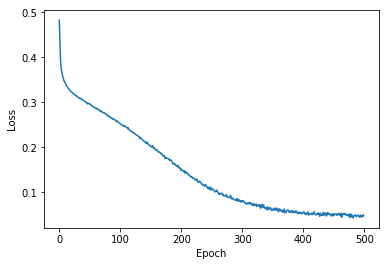
\includegraphics[scale=0.7]{Figures/chapter04/fe_palette_color.png}
	\decoRule
	\caption[Feature Engineering Learning Curve for Color-Based Prediction]{\textbf{Learning Curve for Palette-Color Histogram based Prediction}~~~The depiction shows the loss per training episode for the \acrshort{mlp} trained on histograms of palette images.}
	\label{fig:FeatureEngineeringPaletteColor}
\end{figure}

A simple \acrshort{mlp} with four hidden layers and 128 neurons in each of them was trained on the resulting normalized histograms of palette colors (ReLU activation / sigmoid activation in the final layer). Hyperparameters were optimized and the network was trained for a total of 500 epochs as the learning curve indicated convergence at this point.

\bigskip
\textbf{Curvature prediction based on partial angles} 

Although the accuracies are far from perfect the results appear to be promising. The hit rate for curvature detection is high: 82\% of all bent spears were identified as such. In comparison, this holds for 71\% of the spears affected by rust and 62\% of the violet spears. In contrast, almost all spears that are identified not to be violet are labeled accordingly (96\% specificity), whereas the specificity for rust (65\%) and curvature (67\%) is lower.

\begin{table}[!h]
	\centering
	\resizebox{\columnwidth}{!}{%
	\begin{tabular}{lrrrrrr}
		{} &  False positive &  False negative &  True positive &  True negative &  Sensitivity &  Specificity \\
		\noalign{\smallskip}
		\hline
		\noalign{\smallskip}		
		bent &            0.19 &            0.07 &           0.34 &            0.4 &         0.82 &         0.67 \\
		\noalign{\smallskip}
		\hline
	\end{tabular}%
	}
	\caption[Feature Engineering Curvature Prediction]{\textbf{Curvature Prediction}~~~Performance of curvature prediction based on angles.}
	\label{tab:performance_angle_based}
\end{table}

\begin{figure}[!hb]
	\centering
	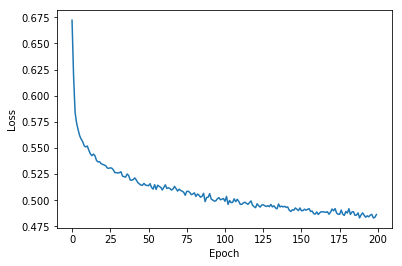
\includegraphics[scale=0.7]{Figures/chapter04/fe_curve.png}
	\decoRule
	\caption[Feature Engineering Learning Curve For Angle Based Prediction]{\textbf{Learning Curve For Angle Based Prediction}~~~The depiction shows the loss per training episode for the \acrshort{mlp} trained on partial angles of the centerline of asparagus spears.}
	\label{fig:FeatureEngineeringCurve}
\end{figure}

\begin{figure}[!htb]
	\centering
	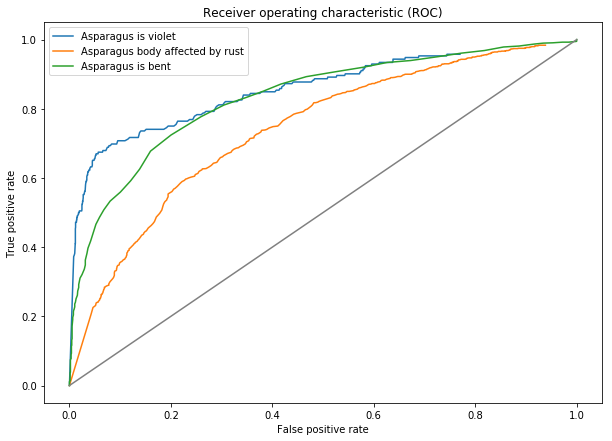
\includegraphics[scale=0.6]{Figures/chapter04/fe_roc.png}
	\caption[Feature Engineering ROC Curve]{\textbf{ROC for MLPs Trained on High Level Features}~~~The depiction shows the \acrfull{roc} for the classifiers that were trained on the features retrieved via feature engineering with \acrshortpl{mlp}. This allows to compare the performance. A larger area under the \acrshort{roc} curve indicates better performance while a curve close to the diagonal line indicates poor results.}
	\label{fig:FeatureEngineeringROC}
\end{figure}

The receiver operating characteristic reveals that the prediction is of better quality for violet and curvature prediction as compared to rust prediction which is reflected in a smaller area under the curve. Possibly this reflects that rather small brown spots were considered rust by some raters but not by others. 

Considering the low agreement in labeling, higher values for the specificity and sensitivity of the classifier were not expected. A likely explanation is that the model generalizes deviating understandings or perceptual color-concepts we had when attributing labels and this affected the reliability of the data. Arguably only little information was discarded by computing the sparse representations that served as an input for training. Information about irregularities in the outline are not reflected in the sparse representation but potentially contribute to the perception of curvature. The same holds for the spatial distribution of colored pixels which might contain additional information regarding rust and violet-detection. However, the major criteria are captured. As \acrshortpl{mlp} have few hyperparameters, they are suitable for non-linear mappings and as the task of mapping high level features to human estimates appears to be rather simple, one could argue that there is little potential to improve the predictive quality using other techniques. By introducing a bias, the sensitivity of the classifier can be adjusted at the cost of more false positives. Here, introducing a bias means that the threshold that is used to convert the floating point outputs of a neural network to booleans that indicate whether a feature is present or not is set to values other than 0.5. The possibility of making the classifier more or less sensitive appears to be a good option to be implemented as a feature for customization by the user in asparagus sorting machines.


\subsubsection{Single-label classification}
\label{subsec:SingleLabel}

In the following chapter, a \acrlong{cnn} is described, which is used for single-label classification on features. The approach was tested on the 13319 hand-labeled data images. 13 models were created, each predicting one feature.~\footnote{The 13 features to predict are fractured, hollow, flower, rusty head, rusty body, bent, violet, very thick, thick, medium thick, thin, very thin, and not classifiable.}

A general model structure was needed as inspiration for the \acrshort{cnn}. For example, the \acrfull{vgg}~networks with varying depth seem to be a good choice for image classification as their \acrshort{vgg}16 won the ImageNet challenge of 2014 and is often implemented for image classification tasks~\citep{hassan2018vgg,vgg2014original}. However, there are two major drawbacks to using them, namely they are slow to train and in need of a lot of memory storage due to their depth and the amount of fully-connected nodes \citep{hassan2018vgg,zhang2015accelerating}. Part of these problems also arise with even deeper networks like ResNet~\citep{resnet2016original,hassan2019resnet}. Thus, AlexNet is chosen as a blueprint for the \acrshort{cnn} because it is small in relation to other networks while still performing comparatively good~\citep{hassan2019alexnet,alexnet2012original,geron2019hands}. As the variance in the data images is relatively small it is assumed that not as many layers are needed as employed in deeper networks like \acrshort{vgg}~\citep{geron2019hands}.
 
\bigskip
The model architecture is roughly based on AlexNet but it is strongly simplified to the level of variability and complexity of the underlying data. The network comprises four hidden layers: a convolutional layer, followed by a pooling layer, a second convolutional layer, and a dense layer. The input is an array of multiple horizontally stacked images with no background removed and reduced by a factor of six. This input is trained on a set of binary labels containing information on whether the respective feature label applies to the current image. The output of the network gives a prediction on each entered image gated by a sigmoid function on a range between zero and one. The rounded integer values of this output give a prediction of the apparent feature label.
For the training phase of the model, the Adam optimizer is used because of its general acceptance as the state of the art optimizer for backpropagation~\citep{bushaev2018adam,kingma2014adam}. As a loss function, binary cross entropy is used as it promises good results for binary single-label classification tasks~\citep{geron2019hands,godoy2018understanding,dertat2017applied}.
 
When training \acrlongpl{ann}, it can be difficult to find clear guidelines on how to implement an architecture such that an optimal training performance is given~\citep{heaton2015aifh,geron2019hands,bettilyon2018classify}. Hence, the idea was to start with the simplest form of a \acrshort{cnn} and then gradually increase the complexity of the network. While AlexNet provides a good baseline for an image classification network, its architecture is still assumed to be unnecessarily complex for the given task. First, the architecture was reduced to the minimum number of layers and parameters needed for a \acrshort{cnn}. Over the period of training optimization, various processing steps and hyperparameters were implemented and compared according to their performance. During this process, the data was split between 12000 samples for training data and 1319 samples of validation data in order to have a reasonable overview on the possible test performance and to directly check for overfitting. The data used as test data was randomly chosen from the whole data set and newly created for every trained model.

\bigskip
In the following the course of the hyperparameters is explained.
 
The batch size was initiated comparatively low with 64 samples per batch but soon adjusted to a value of 512 samples. The larger batch size was implemented in order to guarantee the convergence of the training data, since smaller batch sizes result in jumping gradients, which are not able to converge into any minimum~\citep{bengio2012practical}.
 
Various learning rates were tested during the optimization process. The initial learning rate of 0.003 (which is the standard learning rate for Adam optimizers in Tensorflow~\citep{kingma2014adam,geron2019hands}) was soon found to be too large to guarantee convergence of the algorithm. Thus, the learning rate was decreased and found to be most effective in the range of \(1e^{-5}\) to \(1e^{-8}\). A gradually decreasing learning rate was tested in order to make the training more effective~\citep{bengio2012practical}.~\footnote{In theory, the Adam optimizer already manages learning rate decay~\citep{kingma2014adam}} It does not yield better results and thus a constant learning rate of \(1e^{-5}\) is implemented.
 
Starting with the smallest layer size possible, in the course of time more layers were added. For example, in order to detect the feature fractured one layer for the edge detection should be sufficient. For other, higher-level features, such as bent, more convolutional layers were expected to be more helpful~\citep{geron2019hands}. During the training process, it was settled to a model with the architecture described above.
 
A small number of kernels is used compared to AlexNet since for single-label classification fewer kernels are expected to be needed. The kernel size is picked to be eight $5\times5$ kernels for the first convolutional layer and 16 $3\times3$ kernels for the second convolutional layer. The hidden dense layer consists of 32 neurons. These sizes are assumed to be sufficient, since increasing the number of kernels does not lead to any better results but to overfitting on the training data.
 
Both convolutional layers are built with batch normalization. The gradients were inspected visually and the results give no reason for assuming exploding or vanishing gradients~\citep{pascanu2012understanding}.
 
A next step was to weight the loss function because of the largely unbalanced data~\citep{he2009learning,batista2004study}. However, this did not lead to any changes. The model still tended to make an unbalanced prediction by classifying all values as negative samples. Another idea is to reduce the data set to make the number of images with the regarding feature present even to the number of images where it is absent. This would mean to throw away valuable data, which can otherwise provide information about negative cases to support the model in its training~\citep{batista2004study}. It was decided to keep all data images and instead balance the data by multiplying the minority of samples to match the number of contrary samples. As there was no feature positively exceeding a presence of 50\% in the data, solely positive labels were oversampled. The balancing was only performed on the training data, while the test data was not changed.
 
To prevent overfitting of the negative data samples, \(L_2\) regularization was applied.
 
To improve training performance, some kinds of data augmentation tested \citep{brownlee2019augmentation} like horizontal flipping or small changes in the angle (up to 5\textdegree ) but are not used in the final version.

\bigskip
Around 2700 to 5400 training steps were performed for the training, translating roughly to 120 epochs (with an exception for the feature fractured, which was trained for 60 epochs). Due to the balancing of the data, the number of training data, and therefore the ratio of training steps to epoch, varied when training the \acrshort{cnn} on the different features.

\begin{table}[h]
	\centering
	\resizebox{\columnwidth}{!}{%
	\begin{tabular}{llllll}
		{} & Sensitivity & Specificity & Validation Accuracy & Balanced Accuracy & Training Steps \\
		\noalign{\smallskip}
		\hline
		\noalign{\smallskip}
		fractured & 0.8846 & 0.9976 & 99.32\% & 94.11\% & 2690 \\
		\smallskip
		hollow & 0.7308 (0.7692) & 0.9821 (0.9831) & 97.58\% (97.77\%) & 85.65\% (87.62\%) & 5390 (4270)  \\
		\smallskip
		flower & 0.5603 (0.6983) & 0.8975 (0.8288) & 85.96\% (81.41\%) & 72.89\% (76.36\%) & 4790 (2900) \\
		\smallskip
		rusty head & 0.4311 (0.5210) & 0.8695 (0.8106) & 79.86\% (76.38\%) & 65.03\% (66.58\%) & 4670 (3320) \\
		\smallskip
		rusty body & 0.6420 (0.6400) & 0.7767 (0.8049) & 71.15\% (72.51\%) & 70.94\% (72.25\%) & 2990 (2270) \\
		\smallskip
		bent & 0.6541 (0.6753) & 0.7533 (0.7500) & 71.25\% (71.93\%) & 70.37\% (71.27\%) & 3230 (2470) \\
		\smallskip
		violet & 0.4643 (0.5119) & 0.9652 (0.9452) & 92.45\% (91.00\%) & 71.48\% (72.86\%) & 5150 (3550) \\
		\smallskip
		very thick & 0.9778 & 0.9939 & 99.32\% & 98.59\% & 5390 \\
		\smallskip
		thick & 0.9525 & 0.9688 & 96.41\% & 96.07\% & 3950 \\
		\smallskip
		medium thick & 0.8917 & 0.9249 & 91.87\% & 90.83\% & 4550 \\
		\smallskip
		thin & 0.9399 & 0.9280 & 93.13\% & 93.40\% & 4190 \\
		\smallskip
		very thin & 0.9733 & 0.9579 & 96.13\% & 96.56\% & 4310 \\
		\smallskip
		not classifiable & 0.5217 & 0.9961 & 98.79\% & 75.89\% & 5390 \\
		\noalign{\smallskip}
		\hline
	\end{tabular}%
	}
	\caption[Single-Label CNN Classification Results]{\textbf{Single-Feature Label Classification Results}~~~In this table, the sensitivity, specificity, validation accuracy, balanced accuracy, and the number of training steps are given for each feature model after training on 12000 original hand-labeled data images. The numbers in brackets indicate the best result for the model in relation to its balanced accuracy. For most features, training lasted for 120 epochs. However, the number of data samples (and thus training steps) varies between features because of the data balancing.}
	\label{tab:SingleLabelResults}
\end{table}
 
\begin{figure}[!htb]
	\centering
	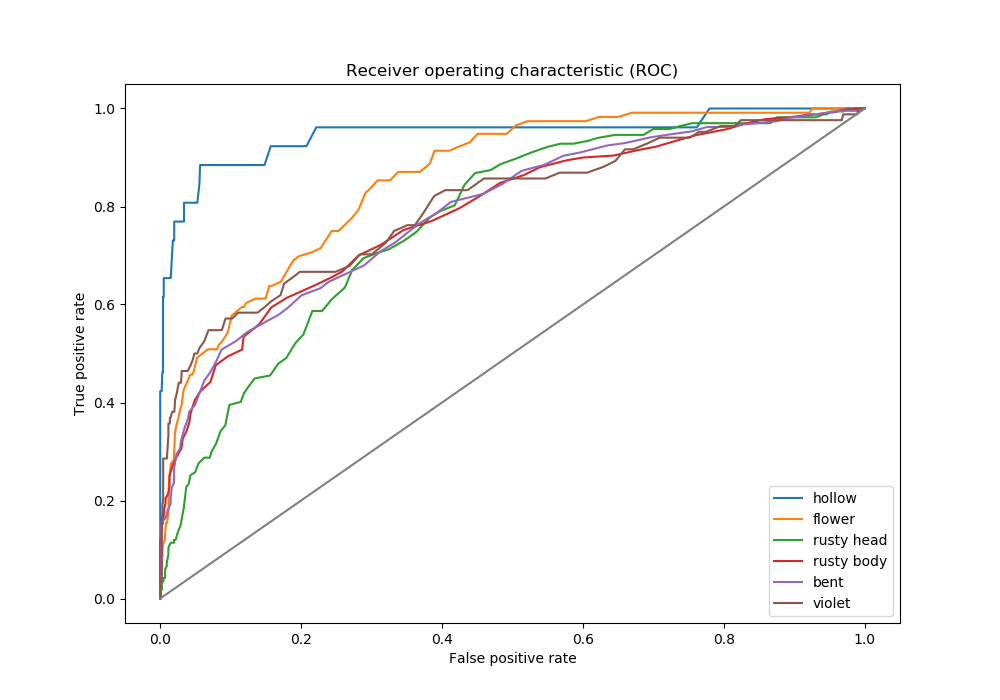
\includegraphics[scale=0.6]{Figures/chapter04/singellabelROC.png}
	\decoRule
	\caption[Single-Label CNN ROC Curve]{\textbf{ROC Curves for Six Feature Models}~~~The figure shows the \acrshort{roc} curves for the six models trained to detect the features hollow, flower, rusty body, rusty head, bent, and violet, respectively. For the features rusty body and bent, the curve is comparatively smooth as their representation is more balanced. The curves are calculated from 1319 data samples.}
	\label{fig:SingleLabelROC}
\end{figure}

The \acrshort{cnn} was trained on 13 features separately, resulting in 13 trained models. For some features, there were no labels in the csv-file but they could be calculated from the parameters length and width of an asparagus. That is, the features very thick, thick, medium, thin, and very thin were all calculated from the thickness measured by the automatic feature extraction algorithm for width, according to the boundaries for each class label (for reference, see \autoref{tab:AsparagusLabels} and \autoref{fig:LabelTree} in \autoref{sec:BackgroundSortingAsparagus}, and further \autoref{subsec:SortingCriteria}). For the feature fractured, the length was set to a threshold of 210 mm, with all asparagus of smaller length labeled as fractured. Additionally, all asparagus labeled as not classifiable was included into the feature fractured. The reason is that fractured asparagus without a head part was previously labeled as not classifiable (see the feature descriptions in~\autoref{subsec:SortingCriteria}). The feature not classifiable was also trained on separately. Further, for all other features, not classifiable samples were removed before training to prevent a bias in the occurrence of false positives.\footnote{Not classifiable asparagus was not sorted for the presence of any other features (see~\autoref{subsec:SortingCriteria}). If a sample is sorted by a model, e.g. that is detecting the presence of feature bent, and the sample shows the sorting criteria, i.e. it is bent, the model will classify it as positive but its feature label will be negative. This will disturb the model and, thus, it was decided to exclude not classifiable samples with an exception for training on feature fractured and for feature not classifiable.}

\begin{figure}[!htb]
	\centering
	\begin{subfigure}{0.3\textwidth}
		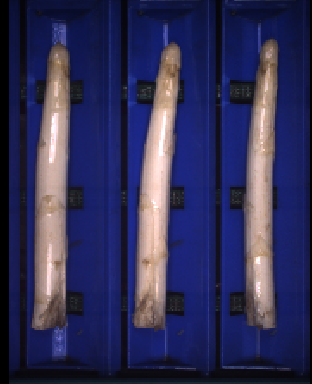
\includegraphics[width=0.9\linewidth]{Figures/chapter04/hollow_falsenegative_01.png}
		\vspace{-5pt}
		\caption{False Negative}
	\end{subfigure}
	\begin{subfigure}{0.3\textwidth}
		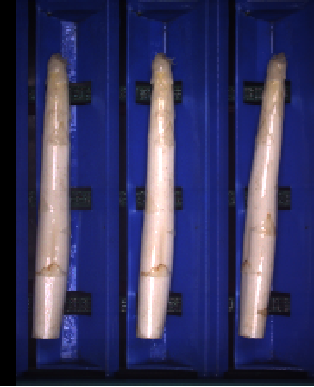
\includegraphics[width=0.9\linewidth]{Figures/chapter04/hollow_falsenegative_02.png}
		\vspace{-5pt}
		\caption{False Negative}
	\end{subfigure}
	\begin{subfigure}{0.3\textwidth}
		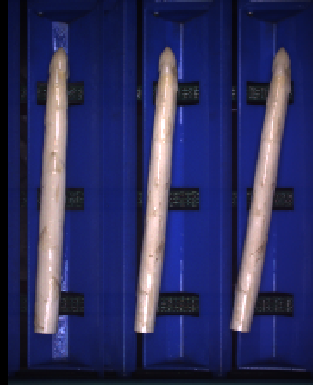
\includegraphics[width=0.9\linewidth]{Figures/chapter04/hollow_falsenegative_03.png}
		\vspace{-5pt}
		\caption{False Negative}
	\end{subfigure}

	\begin{subfigure}{0.3\textwidth}
		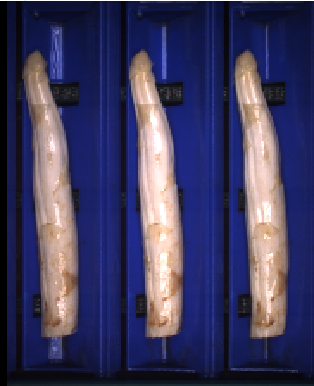
\includegraphics[width=0.9\linewidth]{Figures/chapter04/hollow_falsepositive_01.png}
		\vspace{-5pt}
		\caption{False Positive}
	\end{subfigure}
	\begin{subfigure}{0.3\textwidth}
		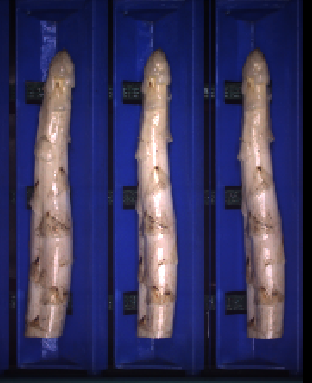
\includegraphics[width=0.9\linewidth]{Figures/chapter04/hollow_falsepositive_02.png}
		\vspace{-5pt}
		\caption{False Positive}
	\end{subfigure}
	\begin{subfigure}{0.3\textwidth}
		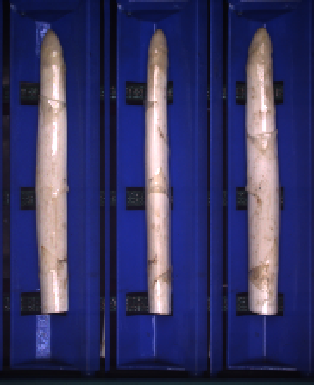
\includegraphics[width=0.9\linewidth]{Figures/chapter04/hollow_falsepositive_03.png}
		\vspace{-5pt}
		\caption{False Positive}
	\end{subfigure}
	\vspace{-5pt}
\caption[Single-Label CNN Example Images Feature Hollow]{\textbf{Feature Hollow}~~~Randomly chosen example images of false negatives and false positives of the feature hollow after 5400 training steps. Image (A) and (C) might have been sorted wrongly as the presence of the feature hollow is not obvious. Of the false positives, image (E) might have also been sorted wrongly, as the vertical line can be seen on the lower part of the asparagus which is a sign for a hollow asparagus (for reference, see the section \nameref{subsec:SortingCriteria}). The thickness of the asparagus might have been an indicator to the model that the feature is present. This can be seen in image (D) which shows a thick asparagus, and image (F) where the asparagus' thickness varies depending on its position.}
    \label{fig:ExampleImagesHollow}
\end{figure}

\begin{figure}[!htb]
	\centering
	\begin{subfigure}{0.3\textwidth}
		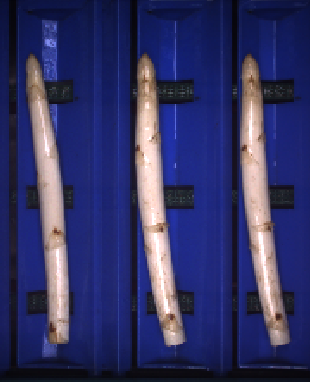
\includegraphics[width=0.9\linewidth]{Figures/chapter04/bent_falsenegative_01.png}
		\vspace{-5pt}
		\caption{False Negative}
	\end{subfigure}
	\begin{subfigure}{0.3\textwidth}
		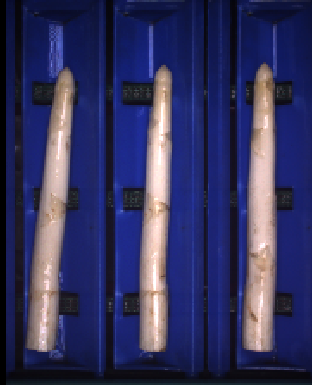
\includegraphics[width=0.9\linewidth]{Figures/chapter04/bent_falsenegative_02.png}
		\vspace{-5pt}
		\caption{False Negative}
	\end{subfigure}
	\begin{subfigure}{0.3\textwidth}
		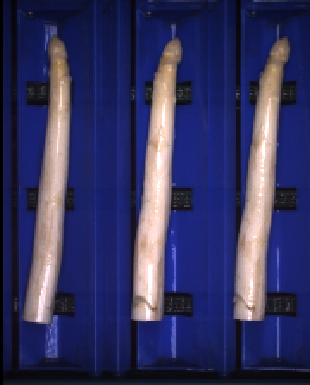
\includegraphics[width=0.9\linewidth]{Figures/chapter04/bent_falsenegative_03.png}
		\vspace{-5pt}
		\caption{False Negative}
	\end{subfigure}

	\begin{subfigure}{0.3\textwidth}
		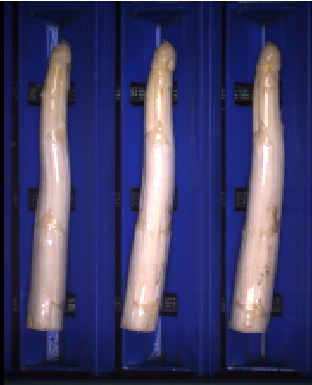
\includegraphics[width=0.9\linewidth]{Figures/chapter04/bent_falsepositive_01.png}
		\vspace{-5pt}
		\caption{False Positive}
	\end{subfigure}
	\begin{subfigure}{0.3\textwidth}
		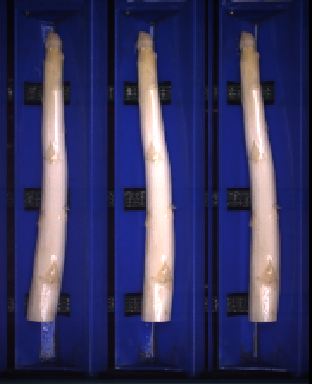
\includegraphics[width=0.9\linewidth]{Figures/chapter04/bent_falsepositive_02.png}
		\vspace{-5pt}
		\caption{False Positive}
	\end{subfigure}
	\begin{subfigure}{0.3\textwidth}
		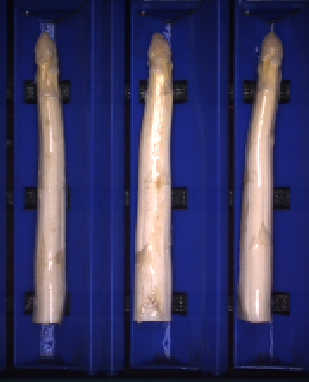
\includegraphics[width=0.9\linewidth]{Figures/chapter04/bent_falsepositive_03.png}
		\vspace{-5pt}
		\caption{False Positive}
	\end{subfigure}
	\vspace{-5pt}
    \caption[Single-Label CNN Example Images Feature Bent]{\textbf{Feature Bent}~~~Randomly chosen example images of false negatives and false positives of the feature bent after 3240 training steps. In all cases the presence of the feature bent is disputed. This becomes evident when comparing false negative and the false positive examples. The difference of both is not clearly evident (see the section~\nameref{subsec:SortingCriteria} for a description of feature bent). It gives the impression that the human labelers did not sort with a strong threshold regarding the feature.}
    \label{fig:ExampleImagesBent}
\end{figure}

\bigskip
In~\autoref{tab:SingleLabelResults} the 13 features are listed on which the \acrshort{cnn} architecture was trained 13 times. It further shows the results for the sensitivity, specificity, validation accuracy, and balanced accuracy of each feature after a certain number of training steps, indicated in the last column of the table.

Sensitivity is a measure to assess the performance of the model in labelling positive samples correctly, while the specificity shows how correctly the model predicts negative samples. The validation accuracy is the accuracy of the validation set which is a representative subset of the entire data set. The balanced accuracy of a feature label is the mean of the sum of its sensitivity and specificity. It represents the accuracy of the feature label if positive and negative samples in the data set were evenly balanced.
Additionally, the performance of six models is calculated in a \acrshort{roc} curve in~\ref{fig:SingleLabelROC}. Models that determine features which indicate the thickness and length, as well as the feature not classifiable are excluded.
In the following discussion, it is referred to the best result of a model (depicted in brackets in~\autoref{tab:SingleLabelResults}) and not the last result.

The results reveal that for every feature, the sum of sensitivity and specificity exceeds 1.  This corresponds to a balanced accuracy over 50\%, which is better than chance level. For all features, the balanced accuracy is above 65\%. Best results are achieved for features that indicate the thickness of an asparagus. The feature very thick reaches the best results with 98\% sensitivity, 99\% specificity, and a balanced accuracy of 98.5\%. Besides features for thickness, the best prediction is observed for the feature fractured, which relies on the parameter length. It reaches a sensitivity of 88\%, a specificity of 99.8\%, and a balanced accuracy of 94\%.
On average, for the hand-labeled features hollow, flower, rusty head, rusty body, bent, and violet a balanced accuracy above 72\% is reached. Feature rusty head performed worst with 52\% sensitivity, 81\% specitivity, and 67\% balanced accuracy. In general, the specificity of all features is relatively high. Most features reach a specificity above 90\%, except for the features flower (83\%), rusty head (81\%), rusty body (80\%), and bent (73\%). For all features, the sensitivity is above 50\%. After visual inspection of test loss and training accuracy, none of the models showed any form of overfitting in their respective range of training steps.
Further, example images of wrong classification are shown for feature hollow in~\autoref{fig:ExampleImagesHollow} and for feature bent in~\autoref{fig:ExampleImagesBent}. Additional example images of false negative and false positive classification for the other features can be found in the appendix in~\autoref{sec:AdditionalSingleLabelCNN}. For feature fractured, training and test loss as well as training and test accuracy are also plotted as an exemplar in the appendix in~\autoref{fig:ExamplePlotsFractured}.\footnote{The log files for accuracy and loss of all models can be found at~\url{https://github.com/CogSciUOS/asparagus}.}
 
\bigskip
The results indicate, that the \acrshort{cnn} architecture is able to learn every feature. Especially features relying on the parameters of length and width achieve a good performance, with both validation accuracy and balanced accuracy above 90\%. The prediction of features like hollow or flower was expected to be more difficult. However, the balanced accuracy of both is above 75\%, with feature hollow even reaching a balanced accuracy of 88\%. This shows that the model predicts them relatively well. Features that depend on color (like rusty body, rusty head, and violet) do not reach equivalent results. It should be further tested whether an increase in model depth might lead to better results for features depending on color or for features depending on a more complex shape (like the feature bent).
 
An inspection of false positive and false negative images at the end of the training process suggests that training performance might be influenced by mislabeled data to a certain extent.
The random images for feature hollow in \autoref{fig:ExampleImagesHollow} propose that the model might use the thickness of an asparagus as an indicator. Some of the samples look like hollow asparagus that could have been labeled incorrectly.
For the feature bent, the randomly selected examples in~\autoref{fig:ExampleImagesBent} might reveal a labeling bias by the human labelers. When the feature is only slightly present, it seems to become a random choice whether the sample was labeled as positive or negative by the human labelers. If true, this can make it difficult for the machine to perform above a certain level of accuracy. It might also be that the difference between the samples is not prominent enough to the model.
Again, these images are just randomly chosen examples and can mean that the model is simply not able to label them correctly. However, the results can also suggest that correct labeling might sometimes be difficult for the model because of an inconsistency in the labeling behavior of the human labelers.
 
On a general note, the architecture of the model is very flexible. It can be applied to many tasks (i.e.\ predicting different features) without much preprocessing of the image data beforehand. Further, the model is quite small, which makes it fast and robust for practical applications. However, instead of having the same architecture for all features, more precise adjustment of each model to its feature is needed.
 
\bigskip
In conclusion, the results of the single-label  \acrshort{cnn} seem promising. Due to a very long debugging phase, there was not enough time to further test and improve the performance of the model. In turn, this means there is still a lot of fine-tuning and possible improvement. A restriction poses the labeling bias of the manually labeled images.

\subsubsection{Multi-label classification}
\label{subsec:MultiLabel}

Building on the standard single-label classification we were further interested in how well a model that predicts several feature labels at the same time performs. A multi-label classification model hereby gets an image as the input and learns to predict the presence or absence of  the feature labels.
For this model, we use a small  \acrshort{cnn} as described below and the features that we labeled by hand. Each of the six features (hollow, flower, rusty head, rusty body, bent and violet) is encoded by a binary output in the target vector, indicating whether the asparagus exhibits the feature in question or not.

\bigskip
Multi-label classification is a useful tool for classification problems in which several classes are assigned to a single input. In contrast to a multiclass classification, where the model is supposed to predict the most likely class for an input, the multi-label classification makes a prediction for each class separately, determining whether the class is present in the image or not. While the different classes are mutually-exclusive in the multiclass classification, they can be related in the multi-label classification. Further, there is no limit on how many classes can be depicted in one image. It is possible that all or none of the classes are present.

Multi-label classification tasks can be thought of as consisting of different sub tasks. Therefore, the problem can be transformed to multiple binary classification tasks. In this transformation, a new model for each feature is trained, which are then combined to give a single output. That means that all features are independent of one another, because they are learned separately. This can be seen as one of the major drawbacks as it is not always clear whether features are related, but in many cases they are.
Therefore, we decided to not only use single-class classification as described in Chapter~\ref{subsec:SingleLabel}but to explore the possibilities of multi-label classification.

A second approach to transform a multi-label classification task is to interpret each possible combination of features as on class. Hereby, the problem is redefined as a multiclass classification task. For a classification problem with six features that means there are \(2^{6} = 64\) classes to be learned. The problems with this approach are, on the one hand, the exponentially increasing number of classes, and on the other hand, the sparsity of samples per class. In many cases, some of the classes are highly underrepresented or even empty. For that reason, we decided not to elaborate this approach further and implement a model for multi-label classification without transforming the task to a multiclass problem.

\bigskip
Inspiration for the model gave a blogpost~\citep{blogpostMulti} which aims to classify images of the MNIST fashion data set in the context of multi-label, rather than multiclass classification. The author altered the data set in such a way that each input image contains four randomly selected items from the MNIST fashion data set. The model then learns to predict which classes are present in the image. The target vector has ten values, one for each class, which are either 0 or 1 depending on whether that class can be found in the input image or not.

This model was chosen as inspiration for two main reasons. Firstly, it tackles a similar problem as ours and the number of classes is similar.

Secondly, the model uses a data set of similar size. Despite the rather small data set in comparison to many other image classification problems, good results with an accuracy of 95-96\% were reached~\citep{blogpostMulti}. This leads us to think, it might be a model with a good complexity for our problem too, as it is complex enough to model the underlying distribution, but not too complex for the medium-sized data set.

\begin{table}[!htb]
	\centering
	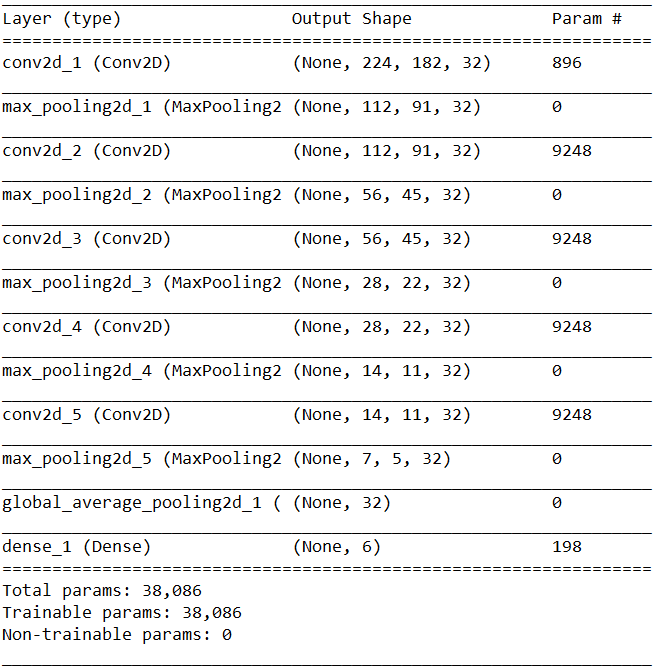
\includegraphics[scale=0.8]{Figures/chapter04/multilabel_structure.png}
	\decoRule
	\caption[Multi-Label Model Structure]{\textbf{Multi-Label Model Structure}~~~The structure of the multi-label classification model is shown. This summary describes which layers are implemented, how the output changes in each layer and how many parameters are trained in each layer and in total.}
	\label{tab:MultilabelStructure}
\end{table}

\bigskip
A classical \acrshort{cnn} was chosen for the multi-label classification task. It consists of five blocks of convolution layers with max pooling layers followed by a global average pooling layer and a dense layer.

In contrast to multiclass classification models, where usually a softmax activation function is used in the last layer together with a categorical cross entropy loss, the multi-label classification model uses a sigmoid activation function and a binary cross entropy loss.

As the input of the model a concatenated image of the three perspectives of each spear is used in order to maximize the information the model gets. This yields input images that look like the three asparagus spears are laying side by side. Further, the images are downscaled by a factor of six to facilitate training (see~\autoref{sec:AsparagusDataSet}).

The output of the model is a vector of length six in which each position encodes one of the six hand-labeled features (hollow, flower, rusty head, rusty body, bent and violet). Each feature can either be present in the input or not, which leads to a 1 or 0 in the target vector, respectively.

Three loss functions are tested to improve the models performance. The first two losses are in-built functions from keras, namely binary cross entropy loss and hamming loss, which uses the fraction of the wrong labels to the total number of labels. Additionally, a custom loss function was implemented, that penalizes falsely classifying a feature as present more than falsely classifying one as absent. The motivation for this custom loss was the fact that the two labels 0 and 1 are highly unbalanced. As previously stated, there are noticeably more 0s than 1s in many classes. To be more precise, the model can reach an accuracy of 77\% by labeling all features as 0. By penalizing this error more, we intended to counteract the unbalanced data set. But at the end, the binary cross entropy loss remains the one with the best results.

Further, it was tested whether regularization would improve the performance of the model on the validation data by preventing overfitting. For this, the model was trained by adding \(L_1\) or \(L_2\) regularization, respectively, to all five of the convolutional layers.  Hereby, a kernel regularization was implemented with a value of 0.01.

\(L_1\) and \(L_2\) regularization can both be interpreted as constraints to the optimization that have to be considered when minimizing the loss term. The main difference between the two is that \(L_1\) regularization reduces the coefficient of irrelevant features to zero, which means they are removed completely. Hence, \(L_1\) regularization allows for sparse models and can be seen as a selection mechanism for features. The inputs to this model are images that consist of a large number of pixels, and additionally a large portion of those pixels are black, because the background was removed. Therefore, it appears to be a good idea to reduce the number of features taken into account in the early layers. \(L_2\) regularization, on the contrary, does not set coefficients to zero, but punishes large coefficients more than smaller ones. This way the error is better distributed over the whole vector.

\begin{figure}[!htb]
	\centering
	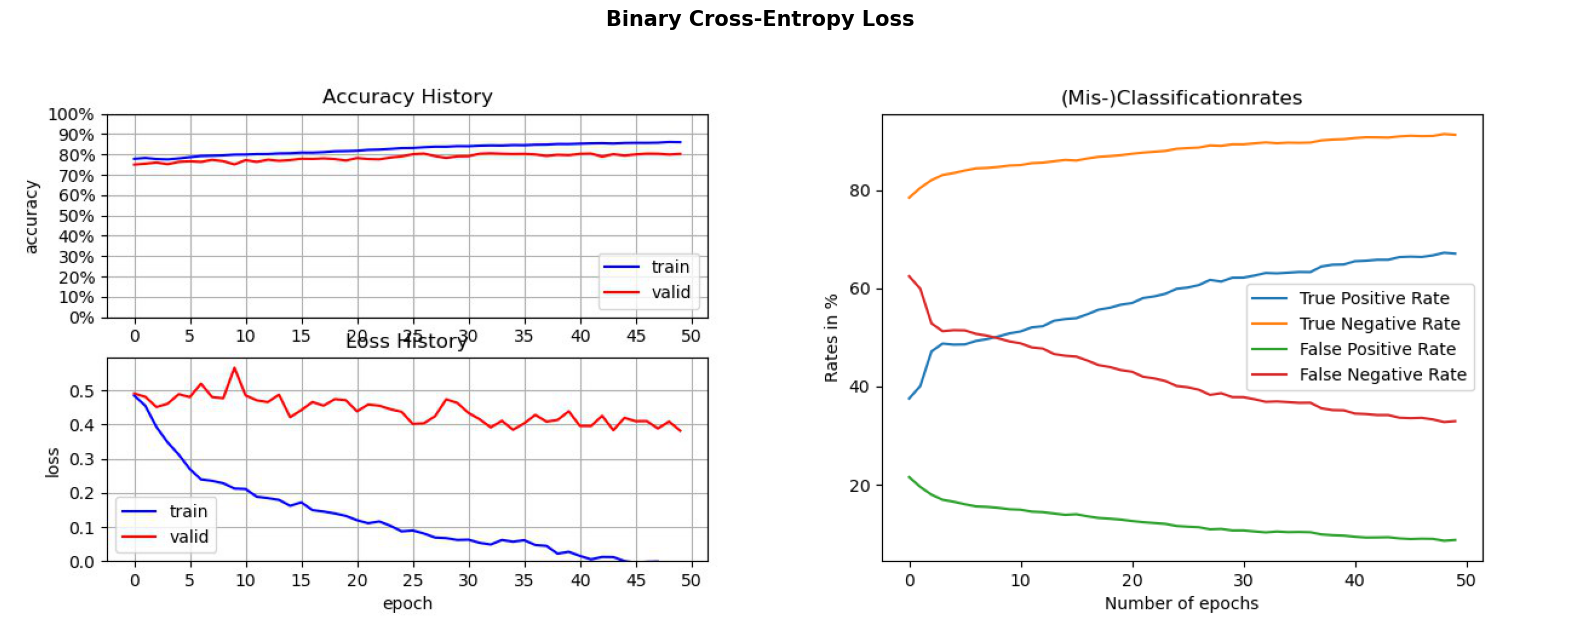
\includegraphics[scale=0.37]{Figures/chapter04/multilabel_crossentropy.png}
	\decoRule
	\caption[Multi-Label Binary Cross-Entropy Loss]{\textbf{Binary Cross-Entropy Loss}~~~These graphs show the evaluation of the training with binary cross-entropy loss. The model was trained over 50 epochs and the accuracy and loss was measured. Further, the false/true positive/negative rates were determined.}
	\label{fig:MultilabelCrossentropy}
\end{figure}

\begin{figure}[!htb]
	\centering
	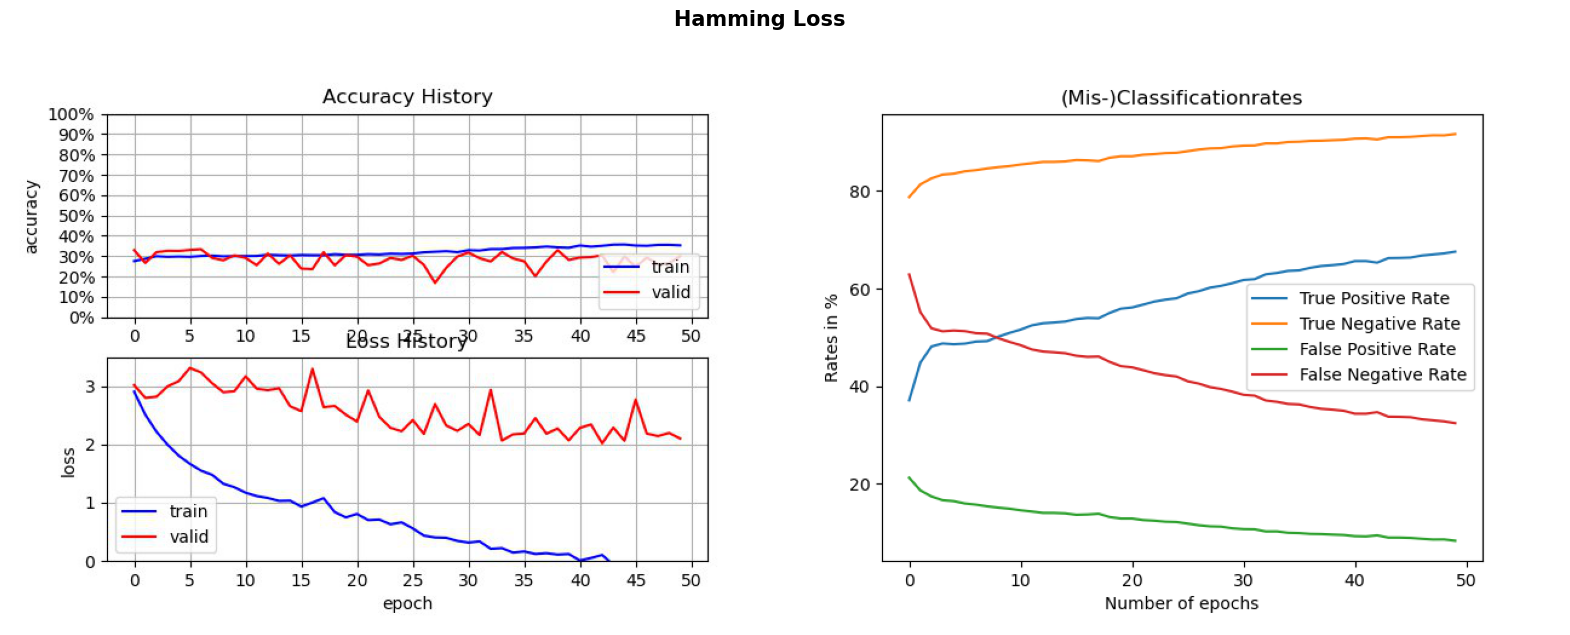
\includegraphics[scale=0.37]{Figures/chapter04/multilabel_hamming.png}
	\decoRule
	\caption[Multi-Label Hamming Loss]{\textbf{Hamming Loss}~~~These graphs show the evaluation of the training with hamming loss. The model was trained over 50 epochs and the accuracy and loss was measured. Further, the false/true positive/negative rates were determined.}
	\label{fig:MultilabelHammingLoss}
\end{figure}

\begin{figure}[!htb]
	\centering
	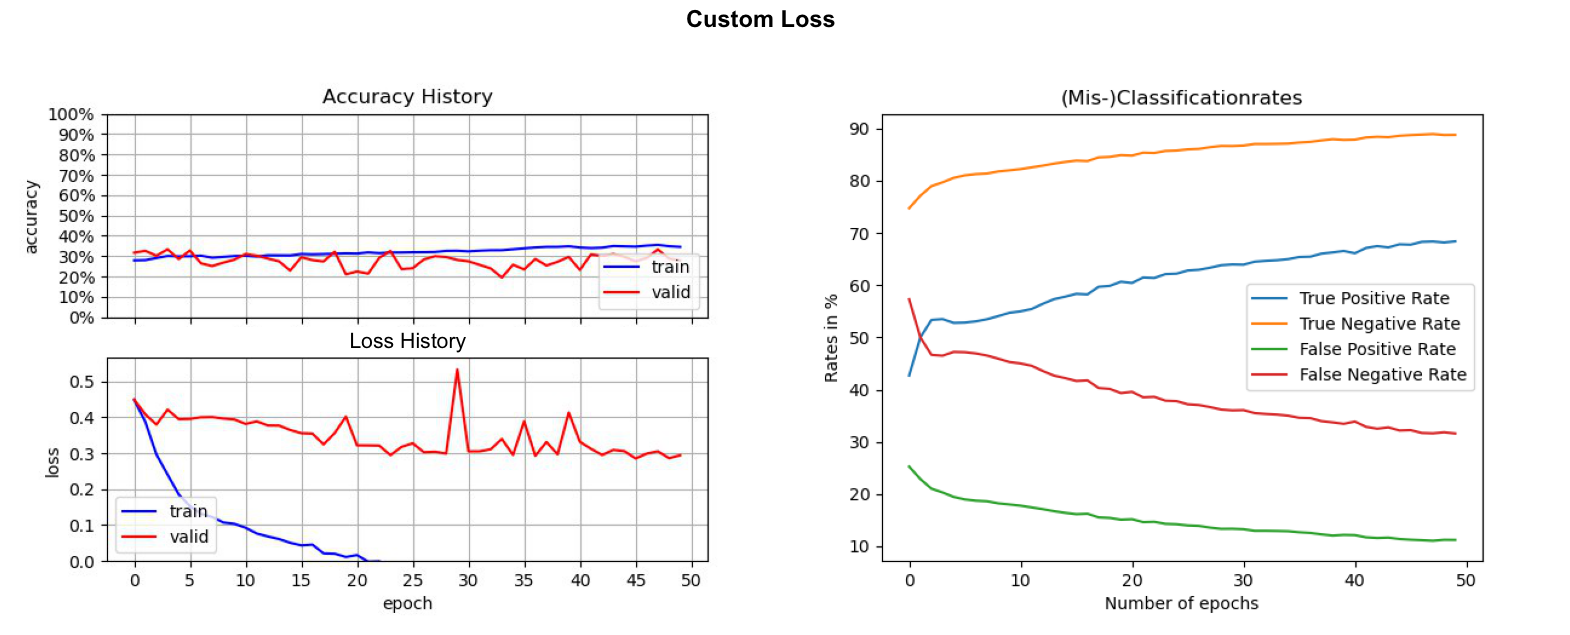
\includegraphics[scale=0.37]{Figures/chapter04/multilabel_costum.png}
	\decoRule
	\caption[Multi-Label Custom Loss]{\textbf{Custom Loss}~~~These graphs show the evaluation of the training with custom loss that punishes falsely classified ones more than falsely classified 0s. The model was trained over 50 epochs and the accuracy and loss was measured. Further, the false/true positive/negative rates were determined.}
	\label{fig:MultilabelCostumLoss}
\end{figure}

\begin{figure}[!htb]
	\centering
	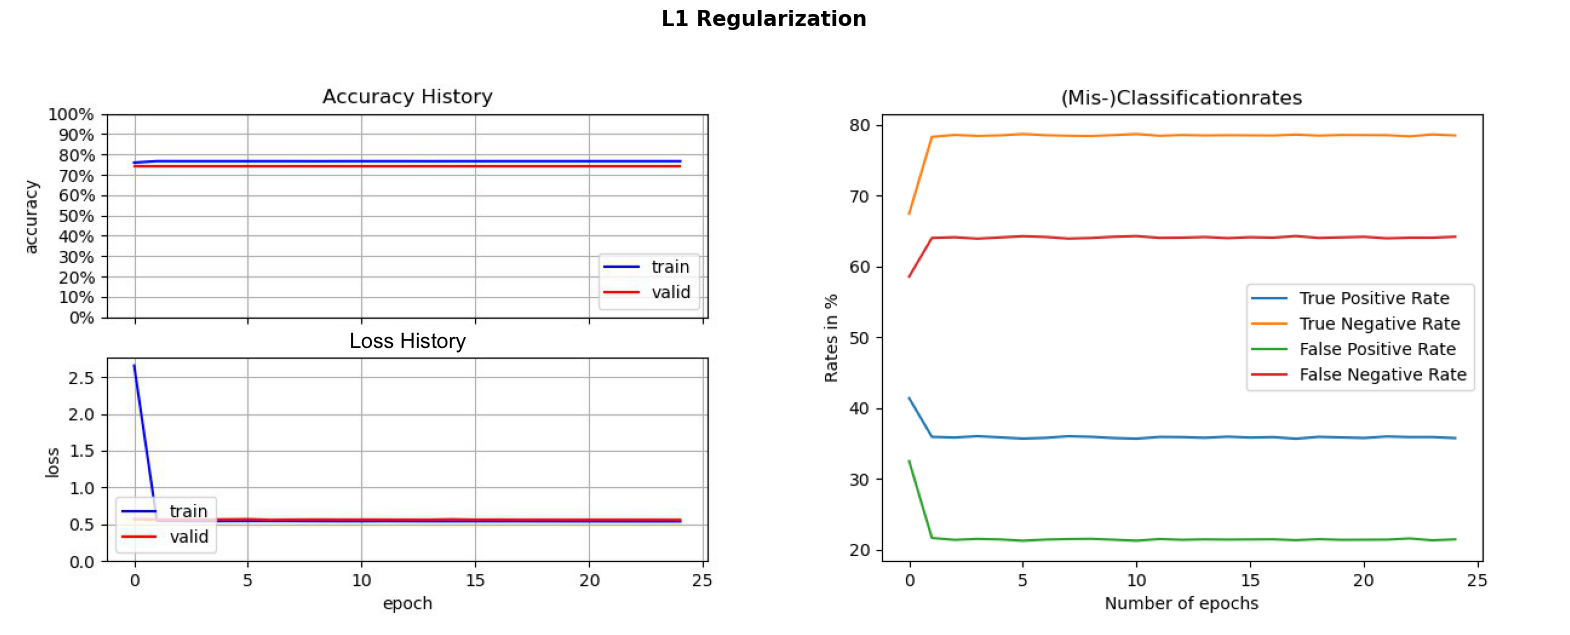
\includegraphics[scale=0.37]{Figures/chapter04/multilabel_L1.png}
	\decoRule
	\caption[Multi-Label \(L_1\) Regularization]{\textbf{\(L_1\) Regularization}~~~These graphs show the evaluation of the training with \(L_1\) regularization. As the loss function the binary cross-entropy loss was used. The model was trained over 25 epochs and the accuracy and loss was measured. Further, the false/true positive/negative rates were determined.}
	\label{fig:MultilabelL1Regularization}
\end{figure}

\begin{figure}[!htb]
	\centering
	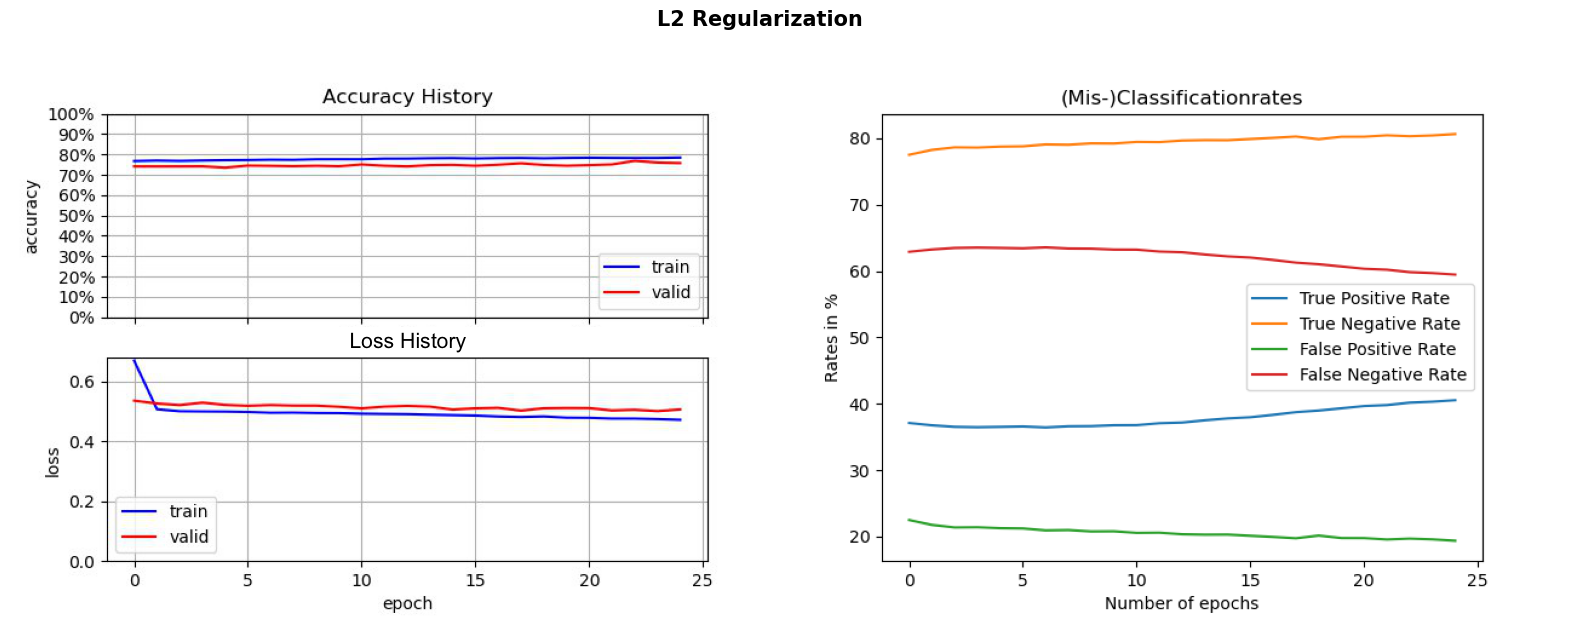
\includegraphics[scale=0.37]{Figures/chapter04/multilabel_L2.png}
	\decoRule
	\caption[Multi-Label \(L_2\) Regularization]{\textbf{\(L_2\) Regularization}~~~These graphs show the evaluation of the training with \(L_2\) regularization. As the loss function the binary cross-entropy loss was used. The model was trained over 25 epochs and the accuracy and loss was measured. Further, the false/true positive/negative rates were determined.}
	\label{fig:MultilabelL2Regularization}
\end{figure}

As shown in \autoref{fig:MultilabelCrossentropy}, \autoref{fig:MultilabelHammingLoss} and \autoref{fig:MultilabelCostumLoss}, all the different approaches explained above show a similar behavior in accuracy and loss values. The training and validation accuracy increase slowly but steadily with the training accuracy always being a little higher than the validation accuracy. The training loss decreases rapidly, while the validation loss only decreases very little and shows random fluctuations. This can be an indicator for overfitting. Usually, \(L_1\) and \(L_2\) regularization are used to prevent overfitting, but in our case it did not improve the results, as shown in \autoref{fig:MultilabelL1Regularization} and \autoref{fig:MultilabelL2Regularization}.

When looking at the sensitivity and specificity, it becomes apparent that both increase during the training process, while the false negative and false positive rates decrease with the same slope. The false positive and false negative rates are mirror images to the true positive and true negative rates with the mirroring axis at the 50\% mark. It can be observed that the rates change rapidly in the first two to four epochs, after which the change progresses slowly in the same direction with no greater disturbances. The model trained with the \(L_2\) loss is an exception as it does not show these large changes in either of the rates.

\bigskip
When comparing the three different loss functions, it is noticeable that the binary cross entropy loss has significantly larger accuracy values than the hamming loss and the costum loss. The values of the binary cross entropy loss start at 75\%, while they start at around 30\% for the other two loss functions. The behavior of the curves and the (mis-)classification rates, however, are very similar in all three approaches. The specificities start off very high with values around 78.46\% for the binary cross entropy loss, 78.73\% for the hamming loss and 74.74\% for the costum loss, and increase further during the training. The highest values are reached with the binary cross entropy loss (91.41\%), closely followed by the hamming loss (91.37\%) and the costum loss (88.75\%). The sensitivity values start off lower, at around 37\% to 42\%, and increase rapidly in the first few epochs, after which the rates proceed to increase but with a narrower slope. They reach values of up to 67.27\% with the binary cross entropy loss, 68.17\% with the hamming loss and 68.17\% with the costum loss. As stated above, the false negative and false positive rates show the same slope but in the opposite direction.

The accuracy values of the models that are trained with \(L_1\) or \(L_2\) regularization, respectively, do not change over the epochs. The same holds for the validation loss. The training loss decreases in the first few epochs and remains stable thereafter.
While the (mis-)classification rates of the model trained with \(L_1\) regularization behave similarly to the ones trained with no regularization, the rates of the model trained with \(L_2\) regularization show a smaller increase and lack the fast change in the first epochs.

The slopes of all curves indicate that the model is learning, because they are increasing in the case of the accuracy, sensitivity and specificity and decreasing in the case of the loss, false positive and false negative rates until the end of training. Hence, one might think that a longer training period will lead to better results. But the training loss decreases very rapidly while the validation loss does not. This suggests overfitting of the model, a problem which gets worse when increasing the training steps. Therefore, a longer training period most likely will not increase performance unless overfitting is prevented. As shown in the result section neither \(L_1\) nor \(L_2\) regularization alone were able to prevent overfitting.

Another common practice that can be tested is the drop-out, in which a certain amount of nodes are left out in different backpropagation steps. This way the model learns to not rely on a small number of nodes but distribute the information between all nodes available. Hence, the coefficients remain smaller. Another method to prevent overfitting is to reduce the model's complexity. A model with fewer parameters to train, is less prone to overfitting. A fitting degree of complexity should be found to model the data sufficiently good without losing the possibility of generalization.

Accuracy alone might not be a good indicator to evaluate a multi-label model~\citep{gibaja2015}. As it highly depends on the loss function, it may have misleading results. This can be seen in the comparison between the three different loss functions. Although the sensitivity and specificity show similar values, the accuracy values suggest that the binary cross entropy loss outperforms the other two loss functions by far. The accuracy of the model trained with the binary cross entropy loss has an accuracy more than twice as high. But when looking at the slope of the curve, it appears that the model with the binary cross entropy loss does not perform better than the other two models. All three have an increase of accuracy of roughly 10\% and a similar sensitivity and specificity. This indicates that the slope of the accuracy function can be considered to evaluate the training process of the model, but the real values should be interpreted with caution.

One thing that comes to attention when looking at the (mis-)classification rates is that the sensitivities are a lot lower than the specificities. A reason for that might be that the positive values are more difficult to learn because they are only sparsely present. The model might have learned that, if the allocation to an output class is not clear, a 0 is the more likely guess.

The \(L_1\) and \(L_2\) regularization both seem to prevent the model from learning all together instead of only preventing overfitting. A reason for that might be that the regularization factor is too high. More experiments should be conducted with varying values to test this hypothesis.

\bigskip
In summary, the model improves its sensitivity and specificity, but it seems like it does so by overfitting the training data. Therefore, the next step should be to prevent the model from overfitting. Afterwards, it should be tested whether additional changes can improve the performance of the model further.


\subsubsection{A dedicated network for head-related features}
\label{subsec:HeadNetwork}

As mentioned before, some features relate to the asparagus heads only. Hence, it was assumed that classification is easiest when training a \acrshort{cnn} on depictions of the respective region of the asparagus. Therefore, a data set that consists only of images of the head area is used. Images of all three perspectives are appended horizontally such that each sample contains the information from all available viewpoints. This is especially important as rust affected spots are sometimes only visible from some angles. The \autoref{fig:HeadExample} shows one sample of rust affected asparagus heads.

\begin{figure}[!htb]
	\centering
	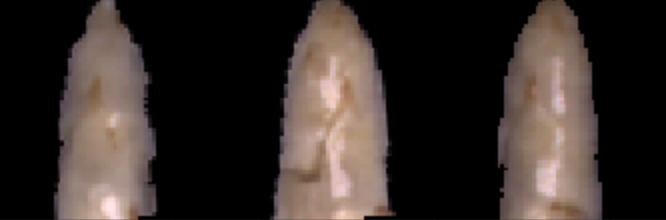
\includegraphics[scale=0.4]{Figures/chapter04/head_example.png}
	\decoRule
	\caption[Head Features CNN Training Sample]{\textbf{Training Sample}~~~The depiction shows a sample for the preprocessed and vertically aligned asparagus heads. Mind that images from all perspectives were stacked horizontally and used as a single input for the \acrshort{cnn}.}
	\label{fig:HeadExample}
\end{figure}

A simple feedforward \acrshort{cnn} was trained on the images. The features flower and rusty head are chosen as target categories. Hence, the  model is another example for multi-label classification. The network comprises the input layer, three convolutional layers with kernel size two, a fully connected layer with 128 neurons as well as the output layer. For the final layer, the sigmoid activation function is applied while the hidden layers have ReLU activations. A dropout layer was added to avoid overfitting. The network was trained using mean squared error \acrshort{mse} as an error function. The development of loss in the learning curve indicates convergence after 40 epochs.

\begin{table}[!hb]
	\centering
	\resizebox{\columnwidth}{!}{%
	\begin{tabular}{lrrrrrr}
		{} &  False positive &  False negative &  True positive &  True negative &  Sensitivity &  Specificity \\
		\noalign{\smallskip}
		\hline
		\noalign{\smallskip}	
		flower     &            0.04 &            0.06 &           0.08 &           0.82 &         0.55 &         0.95 \\
		rusty head &            0.02 &            0.13 &           0.03 &           0.83 &         0.19 &         0.98 \\
		\noalign{\smallskip}
		\hline
	\end{tabular}%
	}
	\caption[Head Features CNN Performance]{\textbf{Performance of Head Features CNN}~~~Performance of the \acrshort{cnn} trained on asparagus heads.}
	\label{tab:performance_measures_head_based}
\end{table}

\begin{figure}[!htb]
	\centering
	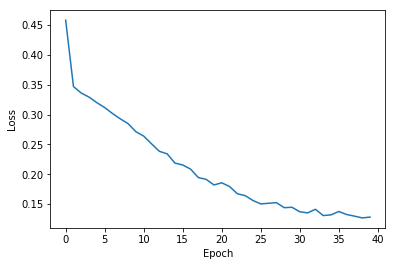
\includegraphics[scale=1.8]{Figures/chapter04/head_curve.png}
	\decoRule
	\caption[Head Features CNN Learning Curve]{\textbf{Learning Curve for the Head Features CNN}~~~The depiction shows the loss per training episode for the \acrshort{cnn} trained on asparagus heads.}
	\label{fig:HeadCurve}
\end{figure}	

\begin{figure}[!t]
	\centering
	\vspace{2cm}
	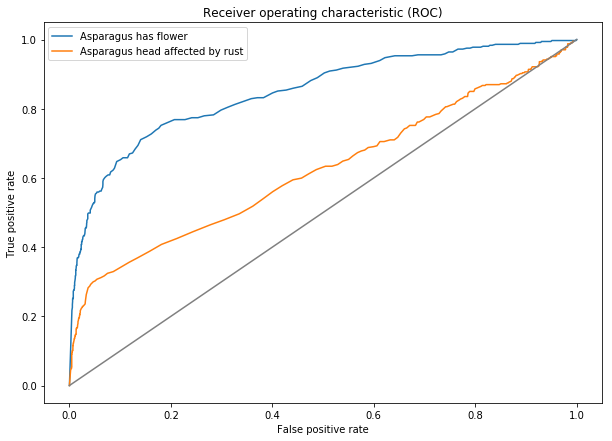
\includegraphics[scale=1.55]{Figures/chapter04/head_roc.png}
	\decoRule
	\caption[Head Features CNN ROC Curve]{\textbf{ROC for the Head Features CNN}~~~The depiction shows the \acrfull{roc} for the predictions of the \acrshort{cnn} trained on asparagus heads. It allows to compare the performance. A larger area under the \acrshort{roc} curve indicates better performance while a curve close to the diagonal line indicates poor results.}
	\label{fig:HeadROC}
\end{figure}

\bigskip
The results for both features show to be highly specific. In contrast, the sensitivity is rather low. Only 55\% of the asparagus spears labeled as flower are identified as such whereas the true positive rate is only 19\% for rusty head. Given the low labeling agreement for these criteria (see \autoref{subsec:Reliability}), these mediocre results are not surprising.

The \acrshort{roc} curve indicates how the classifiers respond to the introduction of a bias and shows the overall prediction quality. The area under the curve is small for the feature rusty head. Beside incongruencies in the labels this is possibly due to the choice of the size of the head region. It might be the case that brown spots in regions other than the cropped head were considered as an indicator for a rusty head when attributing labels. Improvements by increasing the cropped head region appear to be possible.


\subsubsection{From features to labels}
\label{subsec:FeaturesToLabels}

Approximately 200 asparagus spears per class label are pre-sorted and served as ground truth mappings between input images and output class labels. These images were manually annotated with features (see \autoref{sec:ManualLabeling}). This allows to divide the classification process into two steps: In the first step we predict feature values from images and in a second step we predict class labels from those feature values.

\bigskip
This chapter deals with the second step: Using supervised learning to predict 13 class labels based on manually labeled features. These 13 class labels refer to the classes at the asparagus farm Gut Holsterfeld. We built a unified interface to load different models, train them and analyze their predictions. It provides compatibility for scikit-learn as well as for keras models. To explore the data and visualize the predicted results, we built a streamlit app.\footnote{inside code/pipeline in the GitHub repository} This has the advantage that the user can easily load and train a model, select an asparagus spear, see the corresponding pictures and the predicted class label (see \autoref{fig:FeaturetoLabelStreamlitApp}).

\begin{figure}[!htb]
	\centering
	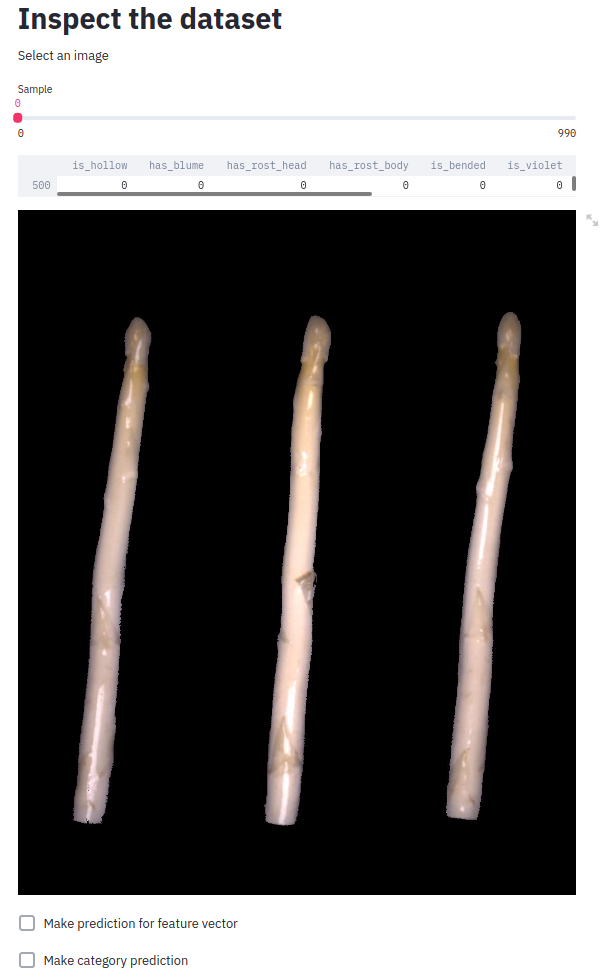
\includegraphics[scale=0.4]{Figures/chapter04/ftl_streamlit_app.png}
	\decoRule
	\caption[Screenshot of Streamlit App]{\textbf{Screenshot of Streamlit App}~~~Screenshot of the streamlit app showing the three images of one asparagus with the corresponding labeled feature.}
    \label{fig:FeaturetoLabelStreamlitApp}
\end{figure}    

\begin{figure}[!htb]
	\centering
	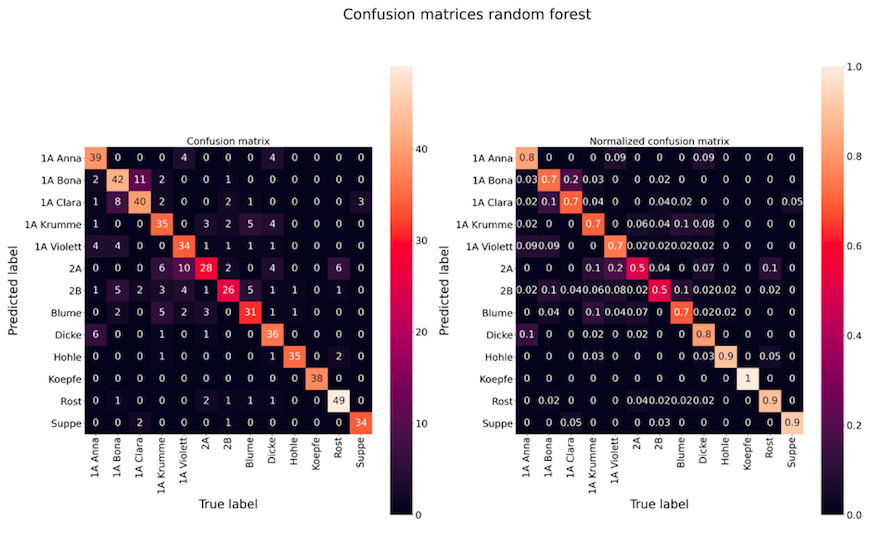
\includegraphics[scale=0.4]{Figures/chapter04/ftl_confusion_recall_random_forest.png}
	\decoRule
	\caption[Random Forest Classifier Confusion Matrices]{\textbf{Random Forest Classifier Confusion Matrices}~~~Confusion matrices showing the absolute and relative number of true positives of the random forest model.}
	\label{fig:FeatureToLabelRandomForest}
\end{figure}

\begin{figure}[!b]
	\centering
	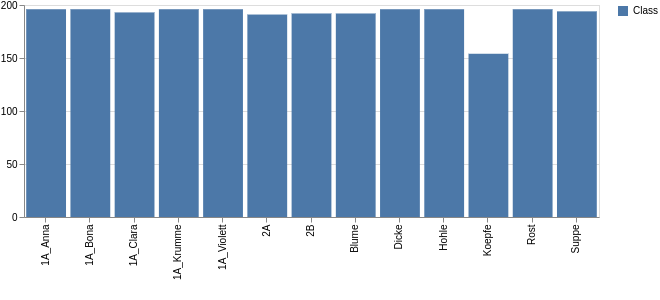
\includegraphics[scale=0.55]{Figures/chapter04/ftl_visualization.png}
	\decoRule
	\caption[Distribution of Class Labels]{\textbf{Distribution of Class Labels}~~~Absolute number of the asparagus spears for which a ground truth class label is available.}
	\label{fig:FeatureToLabelVisualization}
\end{figure}

\begin{table}[!h]
    \centering
    \resizebox{.65\textwidth}{!}{%
    \begin{tabular}{ l r r r r r r }
        {} & precision & recall & f1-score & support \\
        \noalign{\smallskip}
    		\hline
    		\noalign{\smallskip}
1A Anna      & 0.7360      & 0.8936   & 0.8077     & 47      \\
\smallskip
1A Bona      & 0.7000      & 0.7241    & 0.7119     & 58      \\
\smallskip
1A Clara     & 0.7368      & 0.7368   & 0.7368      & 57      \\
\smallskip
1A Krumme    & 0.6667      & 0.6400   & 0.6531     & 50      \\
\smallskip
1A Violet    & 0.6481      & 0.7609   & 0.7000     & 46      \\
\smallskip
2A           & 0.6842      & 0.4643   & 0.5532     & 56      \\
\smallskip
2B           & 0.7179       & 0.5600   & 0.6292     & 50      \\
\smallskip
Blume        & 0.6939      & 0.7556   & 0.7234     & 45      \\
\smallskip
Dicke        & 0.7000      & 0.7955   & 0.7447     & 44      \\
\smallskip
Hohle        & 0.9459      & 0.8974    & 0.9211     & 39      \\
\smallskip
Koepfe       & 1         & 1      & 1        & 38      \\
\smallskip
Rost         & 0.8305        & 0.8909   & 0.8596     & 55      \\
\smallskip
Suppe        & 0.9444      & 0.9189   & 0.9315     & 37      \\
\smallskip
accuracy     & 0.7588      & 0.7588   & 0.7588     & 0.7588    \\
\smallskip
avg          & 0.7696      & 0.7722   & 0.7671     & 622     \\
\smallskip
weighted avg & 0.7591      & 0.7588   & 0.7549     & 622    \\
\noalign{\smallskip}
\hline
    \end{tabular}%
    }
    \caption[Classification Report of the Random Forest Classifier]{\textbf{Classification Report of the Random Forest Classifier}~~The classification report shows key metrics for the trained random forest classifier.}
    \label{tab:FeatureToLabelReport}
\end{table}

%\begin{table}[!ht]
%	\centering
%	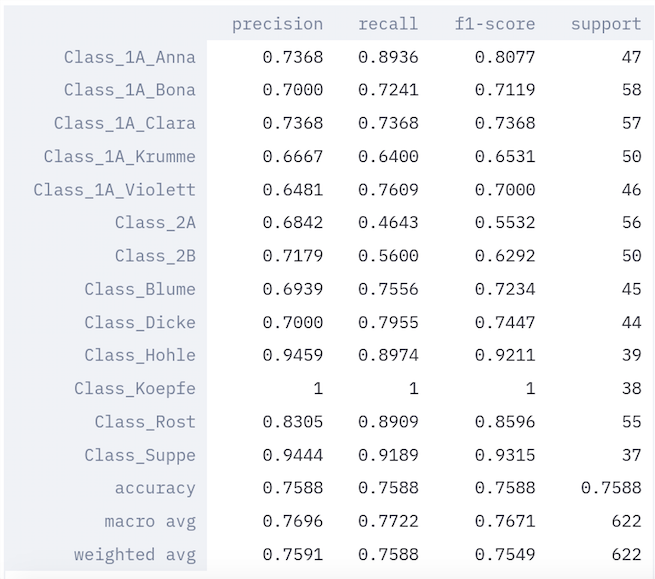
\includegraphics[scale=0.5]{Figures/chapter04/ftl_classification_report.png}
%	\decoRule
%	\caption[Classification Report of the Random Forest Classifier]{\textbf{Classification Report of the Random Forest Classifier}~~~The classification report shows key metrics for the trained random forest classifier.}
%	\label{tab:FeatureToLabelReport}
%\end{table}

The user can also inspect the distribution of the selected data (\autoref{fig:FeatureToLabelVisualization}) and the absolute and relative number of correctly and incorrectly classified asparagus spears in a confusion matrix (\autoref{fig:FeatureToLabelRandomForest}).

The precision and recall are measures on how \enquote{useful and complete} the results are \citep{wiki:precisionrecall}. Precision is the ratio between true positives and the set of all true and false positives, recall the ratio between the true positives and the set of all true positives and false negatives. The confusion matrix (\autoref{fig:FeatureToLabelRandomForest}) gives us insight about which kind of errors the models make. We can observe that classes such as 1A Anna, Dicke, Hohle, Rost, Köpfe, and Suppe can be recalled well (relative recall $\geq$ 0.8), while other classes, such as 2A and 2B have much lower recall ratings (relative recall $\leq$ 0.6). That means that 2A and 2B are the most commonly mislabeled classes (see \autoref{tab:FeatureToLabelReport}).

\bigskip
Two exemplary models were implemented and tested to predict the classes from the features. The first one is a random forest~\citep{breiman2001random} with 100 trees.
Random forests are a popular machine learning approach, because they reach good results in both regression and classification tasks. Further, they are based on decision trees which offer an intuitive interpretation. Although decision trees themselves are powerful tools, they are prone to overfitting. Random forests aim to avoid this problem, while still using the advantages of decision trees, namely that they are flexible, easy to use and fast to train. They do so by training several decision trees on different random parts of the data, after which a majority vote decides on the final output or class. An additional trick is to use a random selection of features for each tree. This reduces the influence of highly correlated features and thereby makes the random forest more robust. 

The second model to predict classes from features is an \acrshort{mlp} with six fully connected layers. It is only implemented to show how to integrate other models, but achieves a similar score as the random forest classifier when trained for 500 epochs (score of 0.76). However, it takes longer to train than the random forest classifier.

The score of 0.76 on the validation set is the accuracy of the random forest classifier, that means that 76\% of the data is predicted correctly –- random guessing would yield an accuracy of 0.08 for uniformly distributed classes, thus the result is satisfying.

\bigskip
Although the results point into the right direction, it would be interesting to see how the selection of features and the agreement on the values of the labeled features influence the performance of the described classifiers. Further work is required to implement the decision process described by the local farmer (see \autoref{sec:BackgroundSortingAsparagus}). One could test if that decision tree based on expert knowledge can outperform the random forest trained on the training samples.


\subsection{Unsupervised learning}
\label{sec:UnsupervisedLearning}

Unsupervised learning are all kinds of machine learning algorithms which deal with unlabeled data. More specifically, they work without a known goal, a reward system or prior training, and are usually used to find structure within data. Dimension reduction algorithms and clustering algorithms have been identified as the two main classes of unsupervised machine learning algorithms which are used in image categorization~\citep{olaode2014}. 

\bigskip
Multivariate data sets are generally high dimensional. However, it is common that some parts of that variable space are more filled with data points than others. A large part of the high dimensional variable space is not used. In order to recognize a structure or pattern in the data, it is necessary to reduce the number of dimensions. For this, both linear- as well as non-linear approaches can be applied. Linear unsupervised learning methods for which also descriptive statistics can be acquired are e.g. \acrfull{pca}, Non-negative matrix factorization, and Independent component analysis~\citep{olaode2014}. Some examples for non-linear approaches are Kernel \acrshort{pca}~\citep{olivier2006semi}, Isometric Feature Mapping,  Local Linear Embedding, and Local Multi-Dimensional Scaling. We employed the linear dimension reduction algorithm \acrshort{pca} as well as well as autoencoders for nonlinear dimension reduction.


\subsubsection{Principal Component Analysis}
\label{subsec:PCA}

\acrlong{pca} was chosen, because it is one of the standard unsupervised machine learning methods. Moreover, it is a linear, non-parametric method and a widespread application to extract relevant information from high dimensional data sets. The goal is to reduce the complexity of the data, by only a minor loss of information~\citep{shlens2014}. Besides being a dimension reduction algorithm, \acrshort{pca} can also be useful to visualize or compress the data, filter noise or extract features.

\bigskip
Our initial aim was to reduce the dimension of our data set for further models. As \acrshort{pca} was applied at the beginning of the data inspection, we also had the aim to visualize our data in a three-dimensional space, in order to get a better understanding of the data distribution. The images that comprise our original data set have a high quality, and instead of only reducing the pixel size, we aimed for reducing the information contained in named depictions by analyzing the principal components in a first step and projecting all relevant images into the lower dimensional space. This information could serve as the input to supervised machine learning algorithms or a simple lookup scheme to retrieve the label of the example with the most similar low dimensional representation.

\bigskip
\acrshort{pca} relies on linear algebra. A general assumption, especially with respect to images, is that large variances are accompanied by important structure. The covariance matrix of the data reveals information about the overall structure and orientation of the data points in the multivariate space. The axis with the largest variance is set as the first principal component. An additional assumption is that the principal components are orthogonal to each other. Therefore, the second principal component is the highest variability of all directions which are orthogonal to the first one~\citep{bohling2006}. The covariance between each pair of principal components is zero, as they are uncorrelated. It generally holds that the higher the eigenvalues are, the more useful they are for the analysis. As eigenvalues specify the variance of the data, higher eigenvalues indicate more relevant features.

The result of a \acrshort{pca} is a representation of the data in a new, smaller coordinate system, which depends on the axes of the largest variance. The dimensionality of this lower coordinate system should depend on the magnitude of the eigenvalues. When plotting the data along the axes of the principal components, it is often easier to understand and interpret the data, than in the original variable space.

It is widely agreed upon that \acrshort{pca} can be a good method to apply dimension reduction on images~\citep{turk1991face,lata2009}.
However, there are several different ways on how to do so. First of all, we performed the \acrshort{pca} on black and white images. When working on black-and-white images, only one data point per pixel is given. Therefore, performing a \acrshort{pca} is less computationally expensive, and finding structure is easier. However, as we need to be able to recognize violet as well as rust, and therefore be able to differentiate between color nuances, it was decided to work on colored images.

\bigskip
There are different possibilities regarding our project which can be considered as useful ways on how to perform a \acrshort{pca}. First, it can be performed on images of different classes at the same time – similar as to capture several images of several people in one database, on which one \acrshort{pca} is performed. In our case this would mean that a \acrshort{pca} is applied to a data set of several input images of all 13 class labels. The second way would be to perform a \acrshort{pca} separately on each group. This way, an ``Eigenasparagus’’ in each group would be calculated, and distances between the Eigenasparagus of different groups could be measured. Thirdly, \acrshort{pca} can be employed feature-wise. In this case, the data set would consist of a collection of images with a certain feature present vs a collection of the same size with the feature absent.

\bigskip
After trying several different approaches, we decided to perform our final \acrshort{pca} on sliced RGB images with background, that are labeled with features by us with the hand-label app, as this seems to yield the best results. An amount of 400 pictures per feature was used to perform a binary \acrshort{pca} for each feature (either the feature is absent or present).

The 200 pictures where a certain feature is present as well as the 200 pictures where a certain feature is absent are extracted loops over the csv-file, where all hand-labeled information is stored as well as the path to the labeled pictures. For each feature a matrix is created, storing 200 pictures with the present feature and 200 pictures without the feature. E.g., m\textunderscore hollow is the matrix created for the feature hollow (shape = 400, img\textunderscore shape[0] $\times$ img\textunderscore shape[1] $\times$ img\textunderscore shape[2]). The first 200 entries in the matrix are pictures of hollow asparagus, the last 200 pictures show asparagus, which is not hollow. These matrices were calculated for the features hollow,  flower, rusty head, rusty body, bent, violet, length and width. The data points of those 400 images in 2D space can be seen in~\autoref{fig:PCAscatter}.

\begin{figure}[!h]
	\centering
	\begin{subfigure}{0.7\textwidth}
		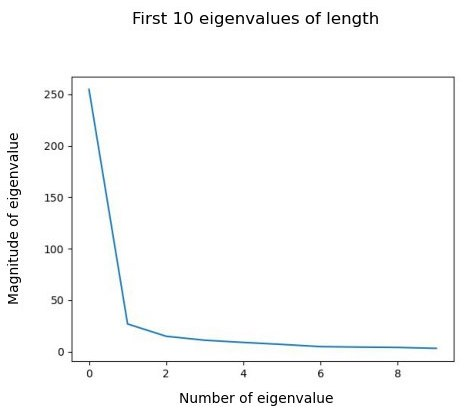
\includegraphics[width=0.9\linewidth]{Figures/chapter04/pca_length_graph.png} 
		\caption{This plots shows the magnitude of the first ten eigenvalues for the feature length.}
	\end{subfigure}
	\vspace{20pt}
	
	\begin{subfigure}{0.9\textwidth}
		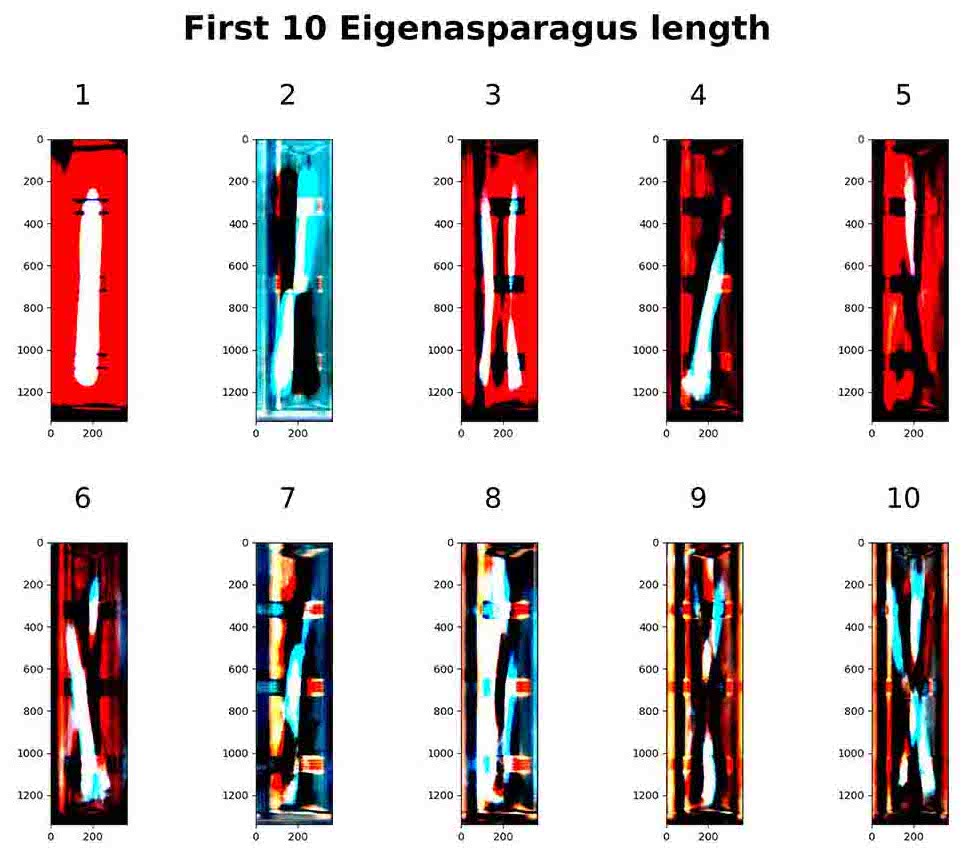
\includegraphics[width=0.9\linewidth]{Figures/chapter04/pca_length.png}
		\caption{These images show the first ten Eigenasparagus of the feature length.}
	\end{subfigure}
	\caption[First Ten Eigenvalues and Eigenasparagus of Feature Length]{\textbf{Eigenvalues and Eigenasparagus of Feature Length}~~~(A) This plots shows the magnitude of the first ten eigenvalues for the feature length. (B) These images show the first ten Eigenasparagus of the feature length.}
    \label{fig:PCAlength}
\end{figure}

%\begin{figure}
%    \centering
%    \subfloat[]{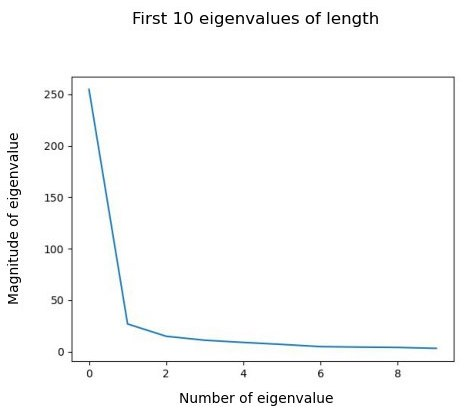
\includegraphics[width=6.5cm]{Figures/chapter04/pca_length_graph}}
%    \qquad
%    \subfloat[]{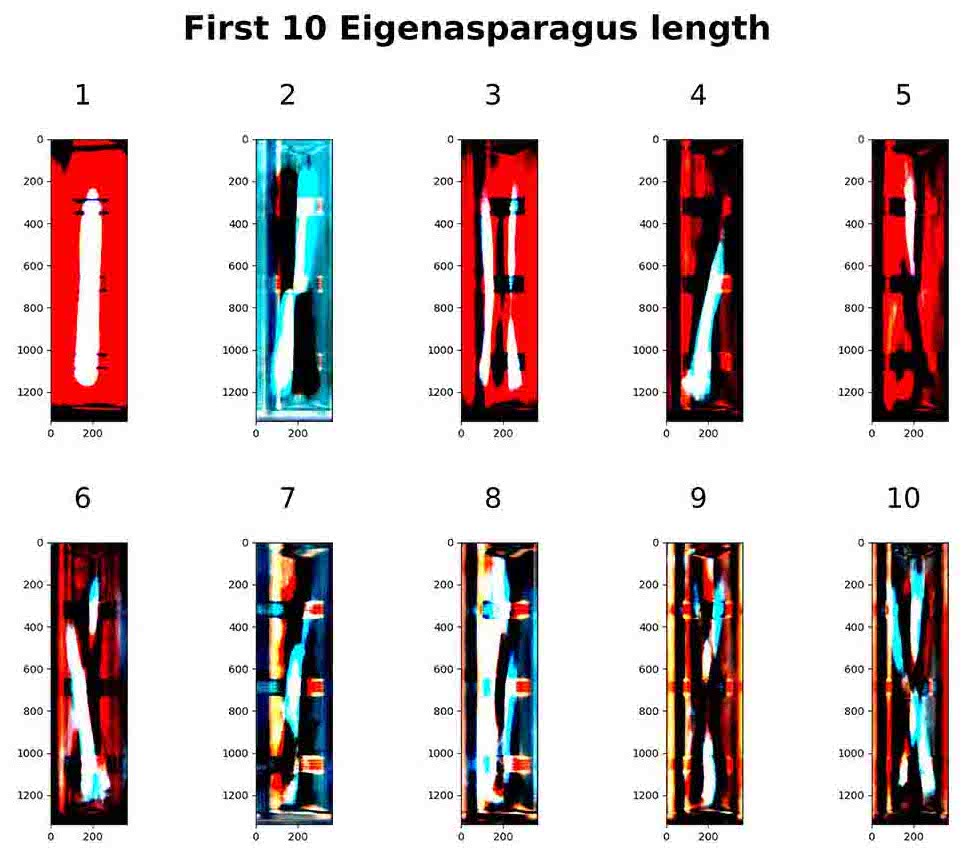
\includegraphics[width=6.5cm]{Figures/chapter04/pca_length}}
%    \caption[First ten Eigenvalues and "Eigenasparagus" of Feature Length]{\textbf{Eigenvalues and "Eigenasparagus" of Feature Length}~~~(A) This plots shows the magnitude of the first ten eigenvalues for the feature length. (B) These images show the first ten “Eigenasparagus” of the feature length.}
%    \label{fig:PCAlength}
%\end{figure}

\begin{figure}[!h]
	\centering
	\begin{subfigure}{0.7\textwidth}
		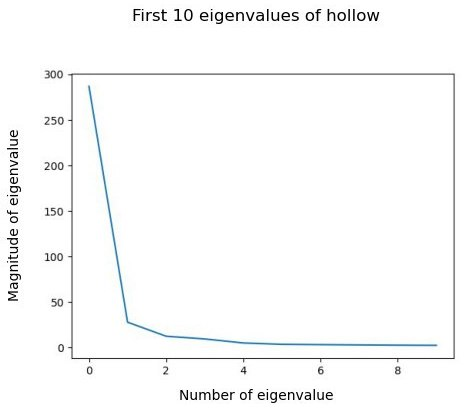
\includegraphics[width=0.9\linewidth]{Figures/chapter04/pca_hollow_graph.png} 
		\caption{This plots shows the magnitude of the first ten eigenvalues for the feature hollow.}
	\end{subfigure}
	\vspace{20pt}
	
	\begin{subfigure}{0.9\textwidth}
		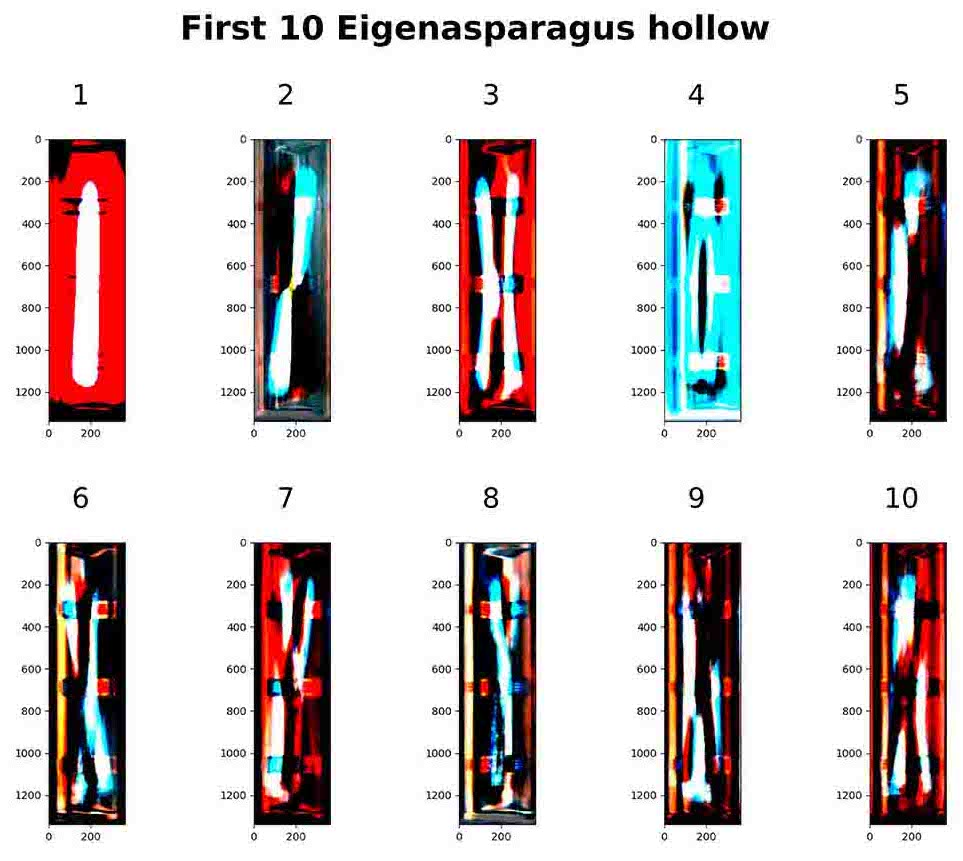
\includegraphics[width=0.9\linewidth]{Figures/chapter04/pca_hollow.png}
		\caption{These images show the first ten Eigenasparagus of the feature hollow.}
	\end{subfigure}
    \caption[First Ten Eigenvalues and Eigenasparagus of Feature Hollow]{\textbf{Eigenvalues and Eigenasparagus of Feature Hollow}}
    \label{fig:PCAhollow}
\end{figure}

%\begin{figure}
%    \centering
%    \subfloat[]{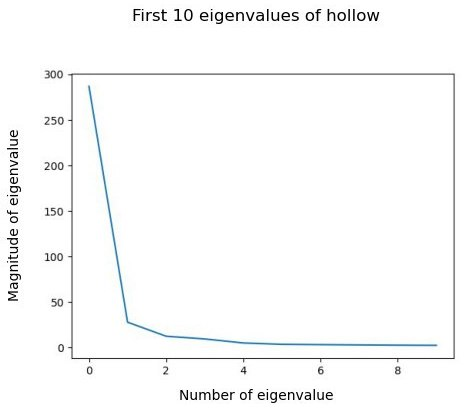
\includegraphics[width=6.5cm]{Figures/chapter04/pca_hollow_graph}}
%    \qquad
%    \subfloat[]{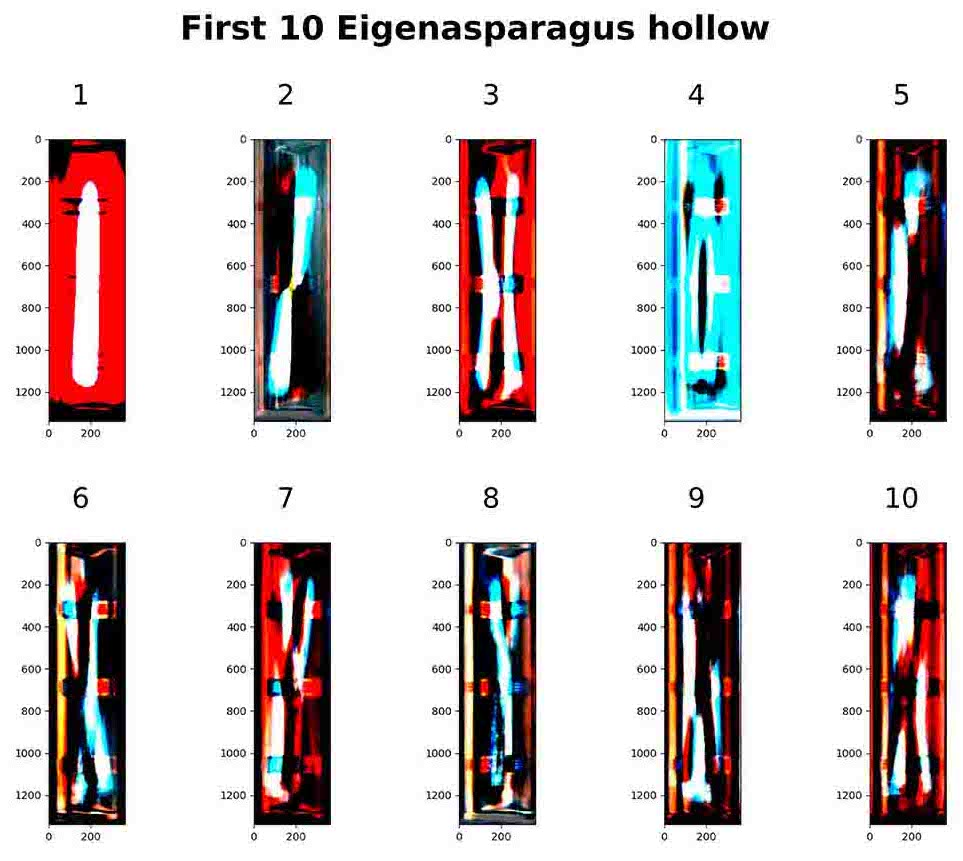
\includegraphics[width=6.5cm]{Figures/chapter04/pca_hollow}}
%    \caption[First ten Eigenvalues and "Eigenasparagus" of Feature Hollow]{\textbf{Eigenvalues and "Eigenasparagus" of feature hollow}~~~(A) This plots shows the magnitude of the first ten eigenvalues for the Feature Hollow. (B) These images show the first ten “Eigenasparagus” of the feature hollow.}
%    \label{fig:PCAhollow}
%\end{figure}

\begin{figure}[!h]
	\centering
	\begin{subfigure}{0.7\textwidth}
		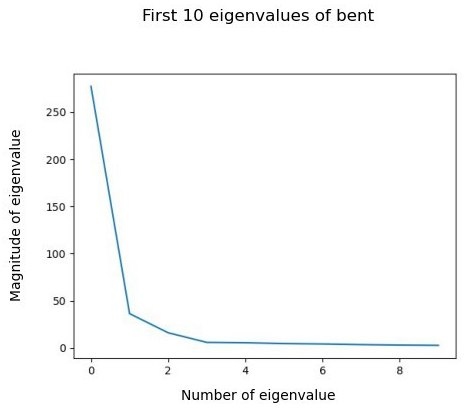
\includegraphics[width=0.9\linewidth]{Figures/chapter04/pca_bent_graph.png} 
		\caption{This plots shows the magnitude of the first ten eigenvalues for the feature bent.}
	\end{subfigure}
	\vspace{20pt}
	
	\begin{subfigure}{0.9\textwidth}
		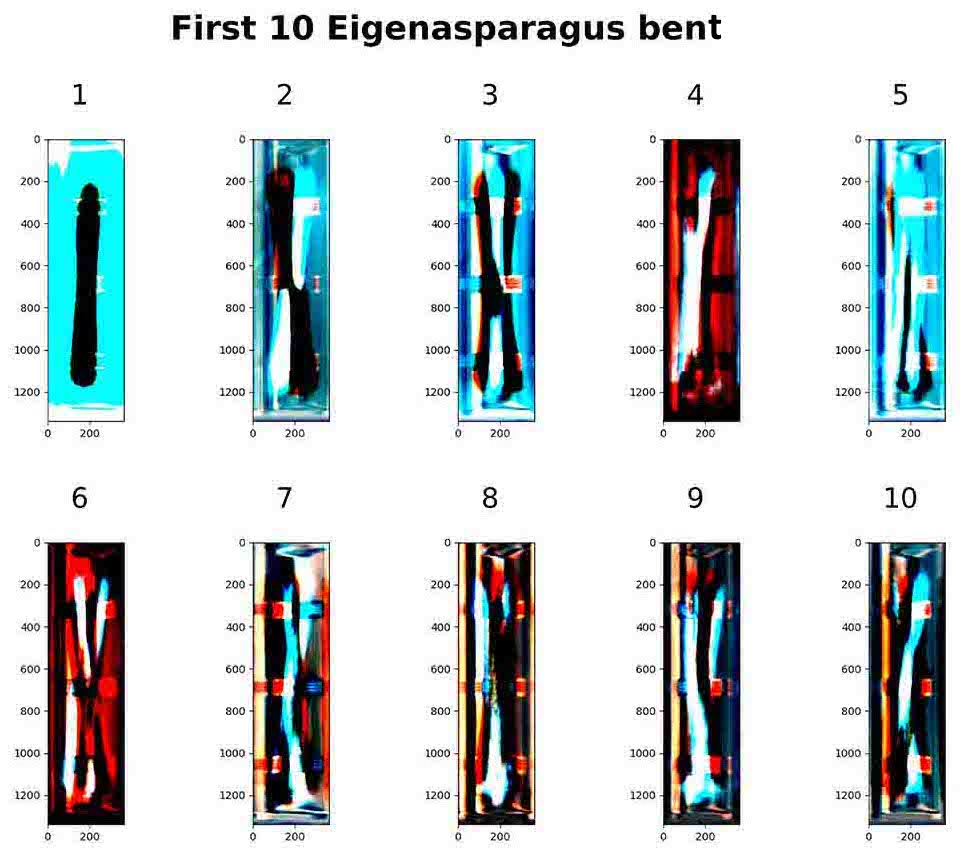
\includegraphics[width=0.9\linewidth]{Figures/chapter04/pca_bent.png}
		\caption{These images show the first ten Eigenasparagus of the feature bent.}
	\end{subfigure}
    \caption[First Ten Eigenvalues and Eigenasparagus of Feature Bent]{\textbf{Eigenvalues and Eigenasparagus of Feature Bent}}
    \label{fig:PCAbent}
\end{figure}

%\begin{figure}
%    \centering
%    \subfloat[]{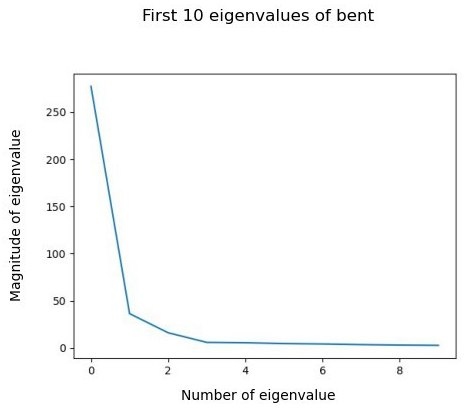
\includegraphics[width=6.5cm]{Figures/chapter04/pca_bent_graph}}
%    \qquad
%    \subfloat[]{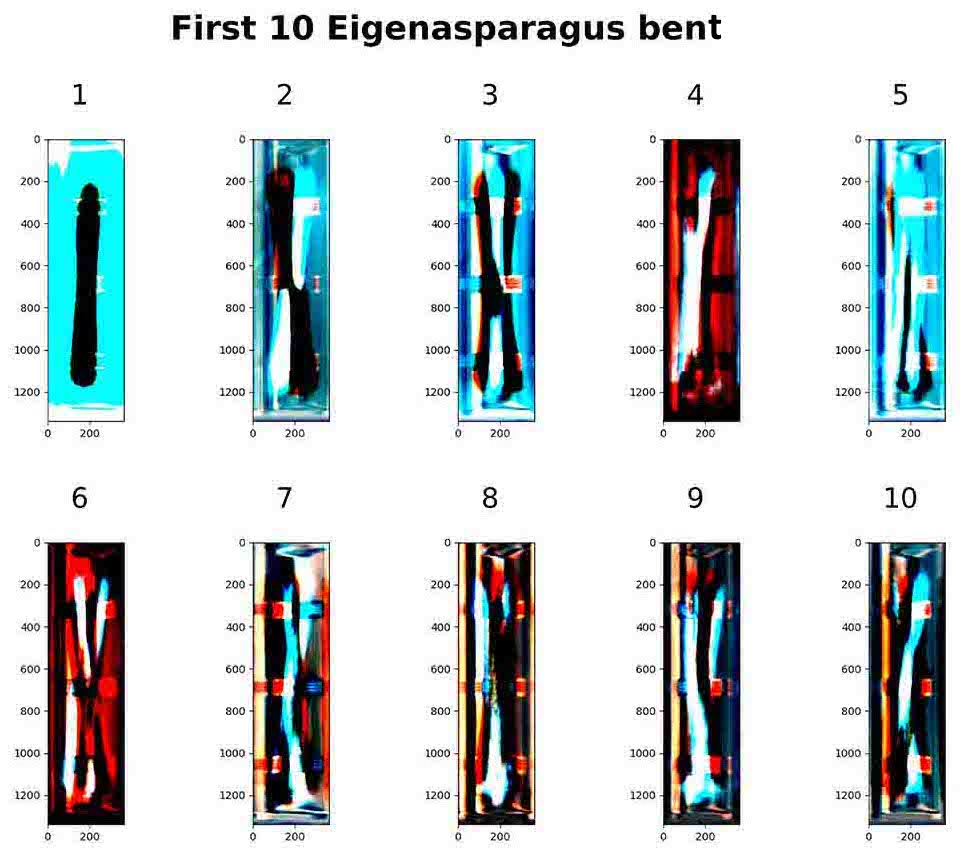
\includegraphics[width=6.5cm]{Figures/chapter04/pca_bent}}
%    \caption[First ten Eigenvalues and "Eigenasparagus" of Feature Bent]{\textbf{Eigenvalues and "Eigenasparagus" of Feature Bent}~~~(A) This plots shows the magnitude of the first ten eigenvalues for the feature bent. (B) These images show the first ten “Eigenasparagus” of the feature bent.}
%    \label{fig:PCAbent}
%\end{figure}

\begin{figure}[!h]
	\centering
	\begin{subfigure}{0.7\textwidth}
		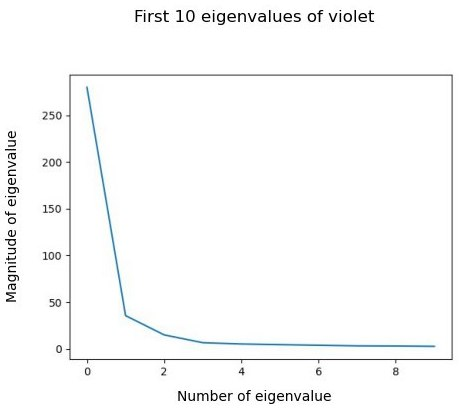
\includegraphics[width=0.9\linewidth]{Figures/chapter04/pca_violet_graph.png} 
		\caption{This plots shows the magnitude of the first ten eigenvalues for the feature violet.}
	\end{subfigure}
	\vspace{20pt}
	
	\begin{subfigure}{0.9\textwidth}
		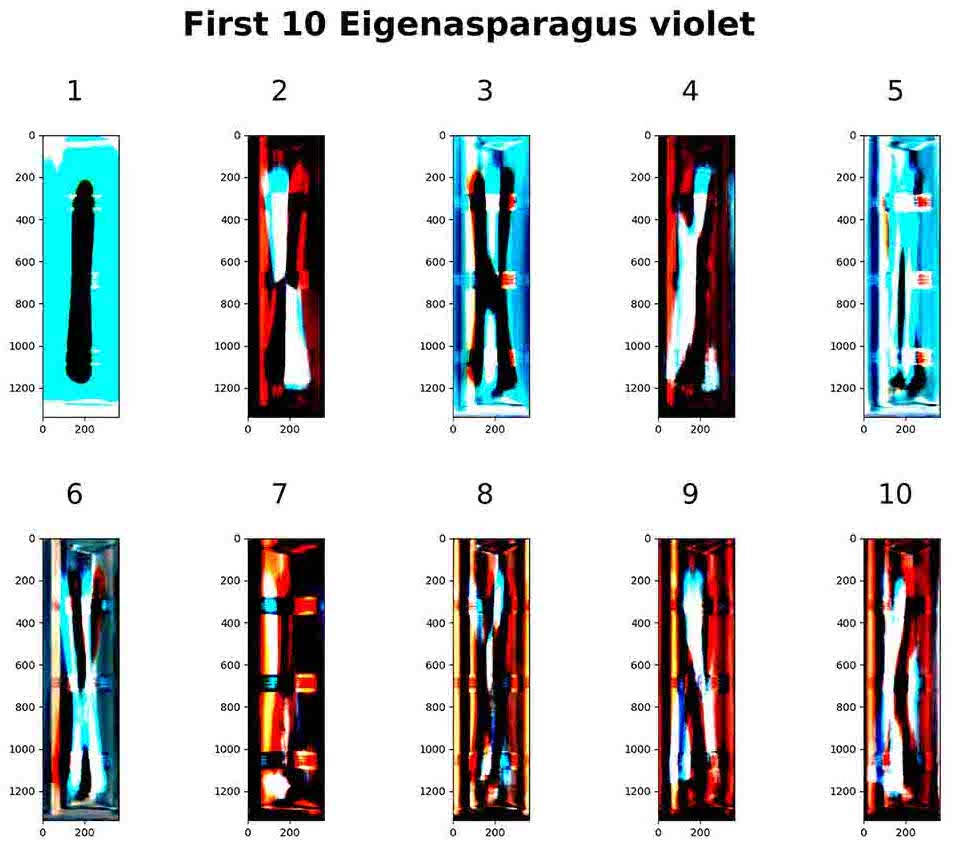
\includegraphics[width=0.9\linewidth]{Figures/chapter04/pca_violet.png}
		\caption{These images show the first ten Eigenasparagus of the feature violet.}
	\end{subfigure}
    \caption[First Ten Eigenvalues and Eigenasparagus of Feature Violet]{\textbf{Eigenvalues and Eigenasparagus of Feature Violet}}
    \label{fig:PCAviolet}
\end{figure}

%\begin{figure}
%    \centering
%    \subfloat[]{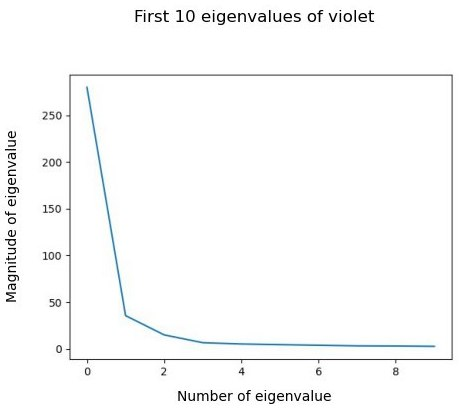
\includegraphics[width=6.5cm]{Figures/chapter04/pca_violet_graph}}
%    \qquad
%    \subfloat[]{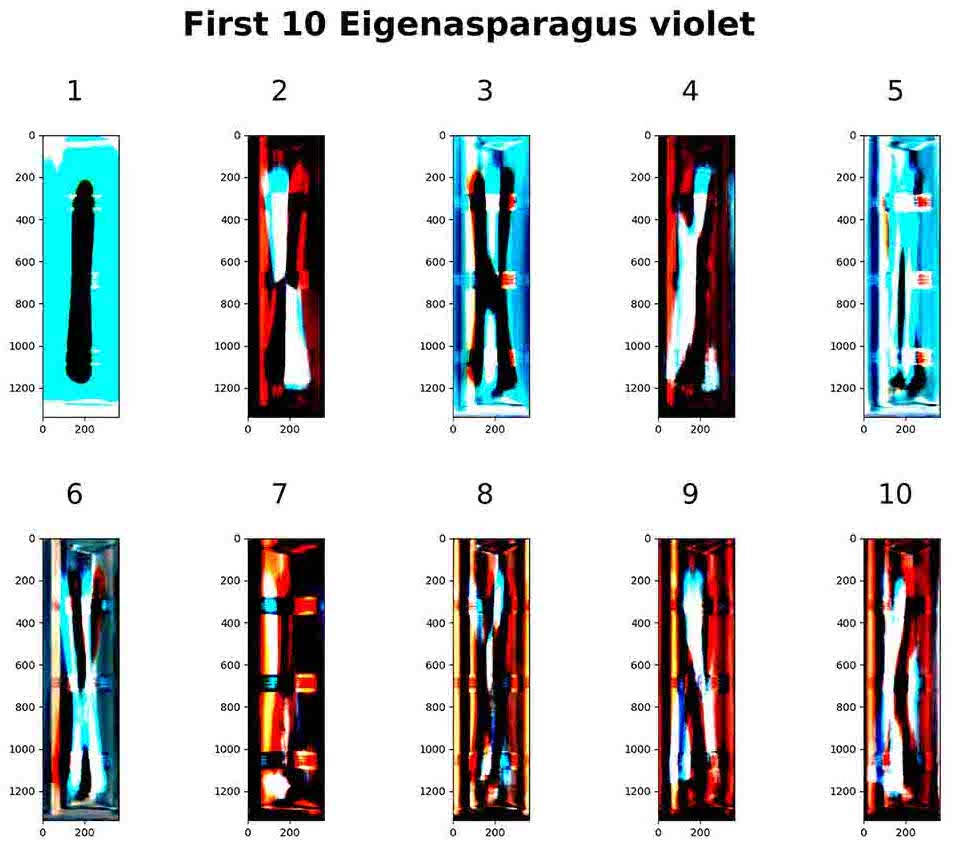
\includegraphics[width=6.5cm]{Figures/chapter04/pca_violet}}
%    \caption[First ten Eigenvalues and "Eigenasparagus" of Feature Violet]{\textbf{Eigenvalues and "Eigenasparagus" of Feature Violet}~~~(A) This plots shows the magnitude of the first ten eigenvalues for the feature violet. (B) These images show the first ten “Eigenasparagus” of the feature violet.}
%    \label{fig:PCAviolet}
%\end{figure}

\begin{figure}[!h]
	\centering
	\begin{subfigure}{0.7\textwidth}
		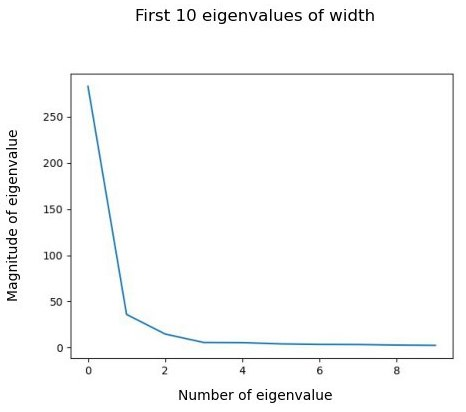
\includegraphics[width=0.9\linewidth]{Figures/chapter04/pca_width_graph.png} 
		\caption{This plots shows the magnitude of the first ten eigenvalues for the feature width.}
	\end{subfigure}
	\vspace{20pt}
	
	\begin{subfigure}{0.9\textwidth}
		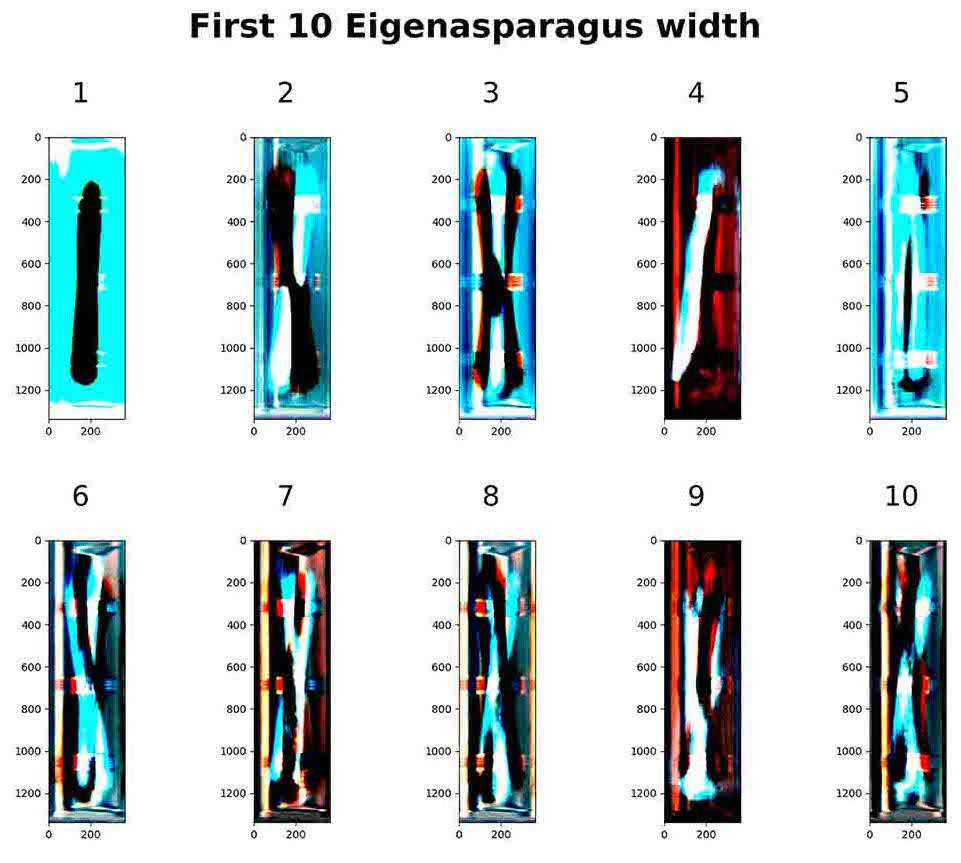
\includegraphics[width=0.9\linewidth]{Figures/chapter04/pca_width.png}
		\caption{These images show the first ten Eigenasparagus of the feature width.}
	\end{subfigure}
    \caption[First Ten Eigenvalues and Eigenasparagus of Feature Width]{\textbf{Eigenvalues and Eigenasparagus of Feature Width}}
    \label{fig:PCAwidth}
\end{figure}

%\begin{figure}
%    \centering
%    \subfloat[]{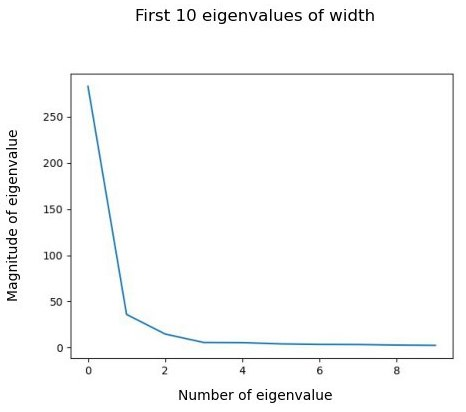
\includegraphics[width=6.5cm]{Figures/chapter04/pca_width_graph}}
%    \qquad
%    \subfloat[]{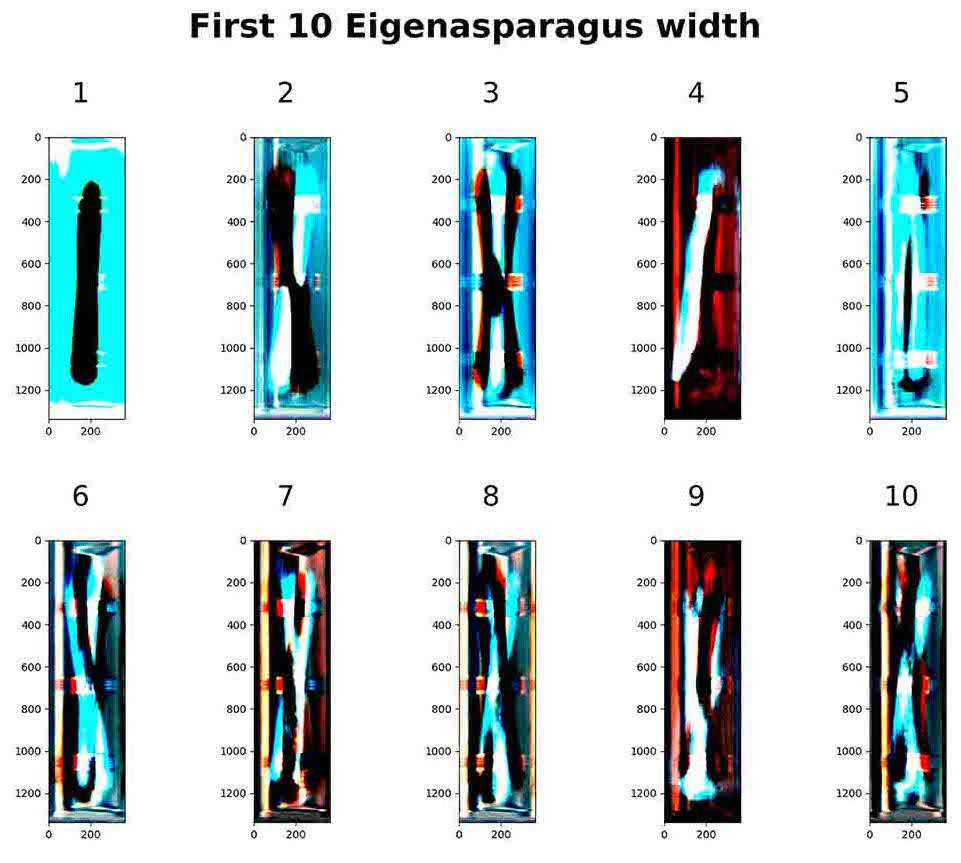
\includegraphics[width=6.5cm]{Figures/chapter04/pca_width}}
%    \caption[First ten Eigenvalues and "Eigenasparagus" of Feature Width]{\textbf{Eigenvalues and "Eigenasparagus" of Feature Width}~~~(A) This plots shows the magnitude of the first ten eigenvalues for the feature width. (B) These images show the first ten “Eigenasparagus” of the feature width.}
%    \label{fig:PCAwidth}
%\end{figure}

\begin{figure}[!h]
	\centering
	\begin{subfigure}{0.7\textwidth}
		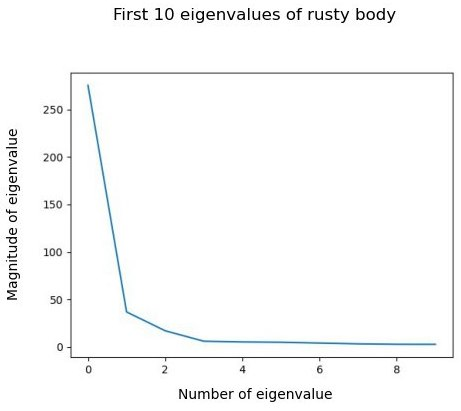
\includegraphics[width=0.9\linewidth]{Figures/chapter04/pca_rustybody_graph.png} 
		\caption{This plots shows the magnitude of the first ten eigenvalues for the feature rusty body.}
	\end{subfigure}
	\vspace{20pt}
	
	\begin{subfigure}{0.9\textwidth}
		\includegraphics[width=0.9\linewidth]{Figures/chapter04/pca_rustybody.png}
		\caption{These images show the first ten Eigenasparagus of the feature rusty body.}
	\end{subfigure}
    \caption[First Ten Eigenvalues and Eigenasparagus of Feature Rusty Body]{\textbf{Eigenvalues and Eigenasparagus of Feature Rusty Body}}
    \label{fig:PCArustybody}
\end{figure}

%\begin{figure}
%    \centering
%    \subfloat[]{\includegraphics[width=6.5cm]{Figures/chapter04/pca_rustybody_graph}}
%    \qquad
%    \subfloat[]{\includegraphics[width=6.5cm]{Figures/chapter04/pca_rustybody}}
%    \caption[First ten Eigenvalues and "Eigenasparagus" of Feature Rusty Body.]{\textbf{Eigenvalues and "Eigenasparagus" of Feature Rusty Body}~~~(A) This plots shows the magnitude of the first ten eigenvalues for the feature rusty body. (B) These images show the first ten “Eigenasparagus” of the feature rusty body.}
%    \label{fig:PCArustybody}
%\end{figure}

\begin{figure}[!h]
	\centering
	\begin{subfigure}{0.7\textwidth}
		\includegraphics[width=0.9\linewidth]{Figures/chapter04/pca_flower_graph.png} 
		\caption{This plots shows the magnitude of the first ten eigenvalues for the feature flower.}
	\end{subfigure}
	\vspace{20pt}
	
	\begin{subfigure}{0.9\textwidth}
		\includegraphics[width=0.9\linewidth]{Figures/chapter04/pca_flower.png}
		\caption{These images show the first ten Eigenasparagus of the feature flower.}
	\end{subfigure}
    \caption[First Ten Eigenvalues and Eigenasparagus of Feature Flower]{\textbf{Eigenvalues and Eigenasparagus of Feature Flower}}
    \label{fig:PCAflower}
\end{figure}

%\begin{figure}
%    \centering
%    \subfloat[]{\includegraphics[width=6.5cm]{Figures/chapter04/pca_flower_graph}}
%    \qquad
%    \subfloat[]{\includegraphics[width=6.5cm]{Figures/chapter04/pca_flower}}
%    \caption[First ten eigenvalues and "Eigenasparagus" of Feature Flower]{\textbf{Eigenvalues and "Eigenasparagus" of Feature Flower}~~~(A) This plots shows the magnitude of the first ten eigenvalues for the feature flower. (B) These images show the first ten “Eigenasparagus” of the feature flower.}
%    \label{fig:PCAflower}
%\end{figure}

\bigskip
For all these features a \acrshort{pca} is calculated by first standardizing the matrix pixel-wise (dimensions: $1340\times346\times3$), calculating the covariance matrix and then extracting the ordered eigenvalues. The principal components are calculated multiplying these eigenvectors with the standardized matrix. The feature space, the principal components and the standardized matrices are saved to later perform a classification function. The highest ten eigenvalues were plotted to visually decide where to set the threshold of how many principal components will be further included. The first ten eigenvalues and the first ten Eigenasparagus for each feature can be seen in \autoref{fig:PCAlength} - \autoref{fig:PCAflower}.

The classification function is a control function, which performs on unseen images and tries to predict if a feature is absent or present. It reads in a new picture of one asparagus, which is not part of the asparagus database, meaning not within the 400 images that were used to calculate the \acrshort{pca}. Then, it searches for the asparagus that is most similar to it in the feature matrices (which are 200 pictures of asparagus carrying the feature, 200 pictures of asparagus without the feature).  This comparison is made with the reduced representation of the original pictures.

In greater detail, the input picture is first centered by subtracting the mean asparagus and then the picture is projected into the corresponding feature-space. That means the picture is translated into the lower dimensional space, in order to compare it to the known 400 pictures. The comparison is made through calculating the distance between the single centered Eigenasparagus and the 400 pictures in the feature space, by using the cdist function of the SciPy package. The smallest distance is considered as the most similar asparagus. If the index of the most similar asparagus is smaller than 200 we know that the feature is present, if it is above 200 the feature is absent. By comparing this to the information of the single asparagus spear, we know if the new asparagus has the same feature as its closest asparagus in the feature space, or not. By doing this for several images, we can already presume if the two features are likely to be easily separable or not. By evaluating this, we have a measure of how well our used principal components capture the distinguishing information of each feature.

\bigskip
The features on which results are given are: Hollow, flower, violet, rusty body, bent, width and length. All features are binary. For the first five features, the manually hand-labeled information was obtained. For the last two features (length and width), the information, which was automatically extracted by the algorithms used in the hand-label app were taken. The decision boundary for the first five therefore depends on our predefined criteria on labeling (see \autoref{subsec:SortingCriteria}). The decision boundary for width was narrower or equal to 20 mm or wider than 20 mm, for length shorter or equal to 210 mm or longer than 210 mm.

There are no results for the feature fractured, even though it is one of the initial main features, as there were only five labeled pictures for this category. Therefore, it was excluded for further analysis. For the feature rusty head, a calculation problem emerged during the process. For an unexplainable reason, there were complex values in the calculation of the principal components. Due to time constraints, this problem was not solved, yet. Therefore, plotting of the feature rusty head is not possible.

By applying the approach for each feature, the eigenvectors, eigenvalues, and principal components for each feature were computed and stored. In all cases, the first principal component is quite high (between 286,94 and 254,78), and drops down rapidly afterwards. The values of the principal components after the fourth principal component are very low ($\leq$~9).

\bigskip
After inspection of the graph of the first ten principal components,  only the first four principal components are used for the analysis, as there is either a sharp drop in the slope after the first four or to maintain continuity between the different features. Following, the corresponding feature space is the space spanned by the first four principal components.

The scatterplots in~\autoref{fig:PCAscatter} show the data of each feature lined up along the axes of the first two principal components of each feature.

\begin{figure}[h]
	\centering
	\includegraphics[scale=0.35]{Figures/chapter04/pca_scatterplot.png}
	\decoRule
	\caption[Feature-Wise Scatterplots]{\textbf{Feature-wise Scatterplots}~~~These scatterplots show the 200 data points where the feature is present in blue and the 200 data points where the feature is absent in orange. The data is projected into a 2D subspace, which is spanned by the first two principal components of each feature.}
	\label{fig:PCAscatter}
\end{figure}

For the classification function, we used the same ten images, to test each feature. The classification works best for the features length and hollow (10/10 classified correctly) and then width (8/10 classified correctly). It performs around chance-level for flower (6/10 classified correctly), violet and rusty body (5/10 classified correctly) and extremely poor for bent (2/10 classified correctly).   

From the images of the first ten principal components, we can visually assume that there is information about the length and shape stored in the first principal component, as a clear asparagus spearpiece can be seen. The following images leave a lot of room for interpretation, about what information is contained there.

We performed the \acrshort{pca} on each feature separately, to extract the principal components of each feature. It is interesting to see that the pictures of the different features are all very similar. One reason for this might be that many of the 400 pictures for each feature are overlapping between the remaining features. Another reason might be, that even though the images vary between features, the general information of all asparagus images is very similar.

\bigskip
From the results of the classification function, one can see that there are large differences between the features in how well our \acrshort{pca} performs (20\% - 100\%).
One reason for this could be that certain features are simply more difficult to distinguish than others. Another reason for this large variation can be that certain features are also more difficult to label consistently (see~\autoref{subsec:AgreementMeasures}), and that the results are due to inconsistencies within the data. One indicator that this is a considerable reason is that the performance of the width and length features, which is information that is not hand-labeled, is very high. Moreover, the poorest results can be observed for the features bent and rusty body. Those are the features, for which the agreement measures show the largest discrepancies between annotators (see~\autoref{subsec:Reliability}).  

\bigskip
Another reason why the results are partly only moderate, is that RGB image data possesses complicated structures, and by representing it in a linear low dimensional feature space, it might be that simply too much information is lost. Even though there are papers reporting good results on \acrshort{pca} on image data~\citep{turk1991face,lata2009}, there are other papers claiming that nonlinear dimension reduction algorithms are needed for this kind of image data~\citep{olaode2014}.


\subsubsection{Autoencoder}
\label{subsec:Autoencoder}

Beside \acrshort{pca}, there are further techniques for dimension reduction. An alternative that can be employed to deduce sparse representations and automatically extract features by learning from examples are autoencoders. Simple autoencoders, in which the decoder and encoder consist of \acrshortpl{mlp}, were already proposed as an alternative to \acrshort{pca} in early days of artificial neural networks when computational resources were still comparatively limited~\citep{kramer1991nonlinear}. Today one can choose from a multitude of network architectures and designs that all have one property in common: A bottleneck layer. For image classification it is common practice to use convolutional autoencoders. There are numerous papers that employed convolutional autoencoders invarious domains. Examples range from medical to aerial radar images~\citep{chen2017deep}. These include not only shallow networks but more recently the benefits of deep autoencoders were demonstrated~\citep{geng2015high}. In addition, more complex architectures combining autoencoders with generative adversarial models were proposed recently~\citep{bao2017cvae}. In many cases the purpose of autoencoders is dimension reduction and feature extraction or in other words the learned latent space of the bottleneck neurons. In other cases, autoencoders are used to map images from one domain to another, for example camera recordings to label-images such that after training a labeled image can be retrieved from the decoder’s output layer\citep{iglovikov2018ternausnet}. In short, there are many possible ways to apply autoencoders and many architectures to realize them.

\bigskip
This motivates the question of how autoencoders work. As mentioned, all autoencoders have a bottleneck layer. If applied for dimension reduction autoencoders are usually used to predict the input, in this case the image, with the input itself. The sparse representation corresponds to the activation of the latent layer for a given input. Autoencoders consist of an encoder that contains the initial layers as well as the bottleneck layer and the decoder that maps the respective latent space back to the image. The desired mapping function of the input to a sparse representation is generated as a side product of the optimization in end to end training, as weights of the decoder are trained such that meaningful features are extracted. The main difference to \acrshort{pca} is that nonlinear functions can be approximated. Feedforward neural networks such as the encoder are non-linear function approximators. Networks with multiple layers are especially well known for establishing named nonlinear correlation. Hence, autoencoders allow for non-linear mappings to the latent space~\citep{kramer1991nonlinear}. This means that in the latter multiple features may be represented in a two dimensional space. It shows that compared to \acrshort{pca} where one dimension typically corresponds to one feature more information can be represented in fewer dimensions. Different properties of the input are mapped to different areas of the latent space. We used \acrfullpl{vae}. In \acrshortpl{vae}, a special loss function is used that ensures features in latent space are mapped to a compact cluster of values. This allows for interpolation between samples by moving on a straight line because regions between points in the latent space lie within the data and hence reconstructions of the decoder are more realistic~\citep{keras2020vae}. Other than that, \acrlongpl{vae} share most properties with regular autoencoders. The location of a point in latent space refers to a compressed representation of the input. These can be interpreted as features of the input.

\begin{figure}[h]
	\centering
	\includegraphics[scale=0.8]{Figures/chapter04/autoencoder_latent_asparagus.png}
	\decoRule
	\caption[Latent Asparagus Space for MLP-VAE and Reconstruction Manifold]{\textbf{Latent Asparagus Space for \acrshort{mlp} -\acrshort{vae} and Reconstruction Manifold}~~~The depiction illustrates the mapping by the encoder and decoder of the \acrshort{vae}: On the left you can see scatterplots illustrating the activation of latent layer neurons for the test data set (the mapping by the encoder). Image-features are mapped to the respective latent asparagus space. There is a scatterplot for each feature of interest where colors indicate positive and negative samples. On the right a manifold of decoded images is shown. The axes relate to the points sampled in latent asparagus space that correspond to the reconstructions (mapping by the decoder).}
	\label{fig:AutoencoderLatentSpace}
\end{figure}

\bigskip
Different \acrlongpl{vae} were tested in the realm of the project. First, a simple \acrlong{vae} with a \acrshort{mlp} as decoder was implemented. The second approach was a comparatively shallow convolutional \acrlong{vae}. The third approach relates to an autoencoder with a deeper encoder that was later used to design the networks for semi-supervised learning. As the third approach is more complex but did not improve the mapping of the properties of asparagus spears to a two dimensional latent asparagus space, the results for the second of named networks are reported here. It was derived from a standard example for \acrlongpl{vae}~\citep{keras2020vae}. The presented results are for a network that comprises two hidden convolutional layers in the encoder and two deconvolutional layers in the decoder.

Similar to the presented way of applying \acrshort{pca}, batches of images that contain only one perspective were used as input to the network. The downsampled data set was used. Images had to be padded as the implementation does not work with inputs of arbitrary shape. The deconvolutional layers of the decoder can only increase dimensionality by an integer factor: The filters that are used for the deconvolution in the given net double the tensor dimensionality. For padded images, this means an increase for the vertical dimension from 34 to 68 and finally to the desired 136 pixels is achieved in the last three layers of the network (impossible for the original height of 134 pixels). The input shape which also defines the shape of the output layer must be divisible by two without remainder twice. Depiction \autoref{fig:AutoencoderLatentSpace} shows the results.

\bigskip
It demonstrates that the features short, thick and thin are mapped to separable clusters. As a tendency curvature correlates with a region in the lower periphery as indicated especially by the deconstruction. The other features (violet, rust and flower) are not mapped adequately and they are not visible in the reconstruction. This shows that only some features of interest were mapped to the latent space and used to decode images. Reconstructions of autoencoders are known to miss many details. Better results could potentially have been achieved using larger input images. The possibility to generate, for example, more or less curved asparagus spears may help to define a clear cut decision boundary and classify images accordingly. As a potential feature for asparagus sorting machines this would allow the user to customize the definition of curvature to the own taste. For this approach to be viable for all features, however, the network performance appears to be insufficient. Some features are poorly separated by the network that was employed on downscaled images.


\subsection{Semi-supervised learning}
\label{sec:SemiSupervisedLearning}

We collected more than 100000 samples. Considering the uniform appearance of the images this represents a substantial amount. However, labels had to be manually generated which was done for only around 10000 samples. As a consequence, there is only a small subset of data with attributed labels. Smaller amounts of labeled data mean that predictions can be successful only if the variance in the source values is limited. Hence, for high dimensional data such as images, sparse representations are desirable. Extracting features automatically instead of relying on manual feature engineering is a strategy that is especially appealing if large amounts of unlabeled data are available. In semi-supervised learning features are extracted from the main input (here images) using unsupervised learning if target labels are unavailable~\citep{keng2017semi}. Hence, semi-supervised learning promises better results by using not only labeled samples but also unlabeled data points of partially labeled data sets.

\bigskip
In the previous chapter, methods and results for unsupervised learning are presented. One example is a convolutional autoencoder. In this section, it is shown how convolutional autoencoders with additional soft constraints in the loss function can be used for semi-supervised learning. Instead of using unsupervised methods to compute another data set of sparse representations and use the latter to predict labels, in semi-supervised learning sparse representations are retrieved and mapped to latent features at the same time~\citep{keng2017semi}. Bottleneck layer activations represent automatically extracted features. For semi-supervised learning one tries to enforce that latent layer activations of autoencoders correlate with the target categories.

\begin{figure}[!htb]
	\centering
	\includegraphics[scale=0.8]{Figures/chapter04/semi_supervised_network.png}
	\decoRule
	\caption[Semi-Supervised Autoencoders Network Structures]{\textbf{Network Structures for Semi-Supervised Learning}~~~The depiction illustrates the network structure for the autoencoders used for semi-supervised learning. Left: The structure for the semi-supervised convolutional \acrlong{vae}. Right: The structure for the semi-supervised convolutional autoencoder. Further explanations can be found in the text.}
	\label{fig:SemiSupervisedNetworkStructures}
\end{figure}

\bigskip
The network structure is derived from the convolutional autoencoder used for unsupervised learning. The feedforward  \acrshort{cnn} is replaced by a network that has proven to be suitable to detect at least some features with sufficient adequacy when trained on heads (see~\autoref{subsec:HeadNetwork}). It comprises three convolutional layers with a kernel size of two in the first and three in subsequent layers as well as 32 kernels each. A max pooling layer with stride two is added mainly to reduce the number of total neurons while maintaining a high number of kernels. Additionally, a dropout layer is added to avoid overfitting. In contrast to other implementations for semi-supervised learning~\citep{keng2017semi} the same network is used for the prediction of labels (when they exist for the current batch) as for the encoder that retrieves the sparse representation for reconstructing images. For the decoder we chose the same one as in the \acrlong{vae} presented in the previous chapter. The effects of a bypass layer that contains neurons not being subject to the label layer loss (see~\autoref{fig:SemiSupervisedNetworkStructures}) were tested. As accuracy did not improve, it was later missed out. Two variations of the network were tested: A convolutional \acrlong{vae} and a \acrlong{vae} for semi-supervised learning.

A challenge results from training with multiple inputs. As deep learning frameworks usually require a connected graph that links inputs to outputs, a trick is used in order to handle that images as well as labels are given as an input. A dummy layer was introduced where all information which is derived from the labels was multiplied by zero. The output vector is concatenated with the bottleneck of the encoder. As it contains no variance, training and more importantly validation accuracies remain unaffected even though information about the categories that are predicted is added on the input side. Nevertheless, the labels are part of the network graph and could hence be used in the loss function.

\begin{figure}[!htb]
	\centering
	\includegraphics[scale=0.35]{Figures/chapter04/semi_supervised_latent_asparagus.png}
	\decoRule
	\caption[Semi-Supervised Convolutional VAE Latent Asparagus Space]{\textbf{Latent Asparagus Space for Semi-Supervised CNN-VAE}~~~The depiction illustrates the mapping by the encoder and decoder of the \acrlong{vae} with additional constraints in the loss function for semi-supervised learning: On the left one can see scatterplots illustrating the activation of latent layer neurons for the test data set (the mapping by the encoder). Image-features are mapped to the respective latent asparagus space. Mind that there is a scatterplot for each feature of interest where colors indicate positive and negative samples. On the right, a manifold of decoded images can be found. The axis relates to the points sampled in latent asparagus space that correspond to the reconstructions (mapping by the decoder).}
	\label{fig:SemiSupervisedLatentSpace}
\end{figure}

A custom conditional loss function is used. If labels are present for the current batch the costum loss is equal to a combined loss that comprises the reconstruction loss and the label loss. Here, reconstruction loss refers to the pixel-wise loss that is used for the main task of the network - namely mapping of input images back to the same images (fed into the network as target values to the output layer). The label loss is used with the goal of mapping label layer activations to the actual labels. It is low if activations in the sigmoid transformed label layer match the target values i.e. the sum of the error layer is low. The loss that is due to labels is multiplied by a custom factor (k). In addition it is defined such that it scales with the current pixel-wise reconstruction loss and converges to a constant (c). These values were chosen aiming for an increase of the contribution of the label loss to the combined loss especially in late stages of training.

\begin{table}[!htb]
	\centering
	\resizebox{\columnwidth}{!}{%
	\begin{tabular}{lrrrrrr}
		{} &  False positive &  False negative &  True positive &  True negative &  Sensitivity &  Specificity \\
		\noalign{\smallskip}
		\hline
		\noalign{\smallskip}
		bent     &            0.04 &            0.37 &           0.04 &           0.55 &         0.10 &         0.94 \\
		violet     &            0.00 &            0.08 &           0.00 &           0.92 &         0.00 &         1.00 \\
		rusty body &            0.14 &            0.27 &           0.20 &           0.39 &         0.42 &         0.73 \\
		fractured         &            0.00 &            0.02 &           0.00 &           0.98 &         0.00 &         1.00 \\
		thick         &            0.00 &            0.07 &           0.00 &           0.93 &         0.00 &         1.00 \\
		thin          &            0.00 &            0.14 &           0.16 &           0.70 &         0.54 &         0.99 \\
		\noalign{\smallskip}
		\hline
	\end{tabular}%
	}
	\caption[Semi-Supervised Convolutional VAE Performance]{\textbf{Convolutional VAE Performance}~~~Performance of the semi-supervised convolutional \acrshort{vae}.}
	\label{tab:performance_convolutional_vae}
\end{table}

\begin{table}[!htb]
	\centering
	\resizebox{\columnwidth}{!}{%
	\begin{tabular}{lrrrrrr}
		{} &  False positive &  False negative &  True positive &  True negative &  Sensitivity &  Specificity \\
		\noalign{\smallskip}
		\hline
		\noalign{\smallskip}
		bent     &            0.02 &            0.34 &           0.07 &           0.57 &         0.18 &         0.96 \\
		violet     &            0.00 &            0.08 &           0.00 &           0.92 &         0.00 &         1.00 \\
		rusty body &            0.23 &            0.19 &           0.28 &           0.30 &         0.59 &         0.57 \\
		fractured         &            0.00 &            0.01 &           0.01 &           0.97 &         0.57 &         1.00 \\
		thick         &            0.00 &            0.06 &           0.00 &           0.93 &         0.04 &         1.00 \\
		thin          &            0.02 &            0.07 &           0.23 &           0.68 &         0.76 &         0.97 \\
		\noalign{\smallskip}
		\hline
	\end{tabular}%
	}
	\caption[Semi-Supervised Convolutional Autoencoder Performance]{\textbf{Convolutional Autoencoder Performance}~~~Performance of the Semi-Supervised Convolutional Autoencoder.}
	\label{tab:performance_semi_supervised_autoencoder}
\end{table}

\bigskip
The results for the semi-supervised \acrlong{vae} are illustrated in~\autoref{tab:performance_convolutional_vae} and visualized by~\autoref{fig:SemiSupervisedLatentSpace}. As one can immediately see, the feature thin was adequately mapped to a decisive region in latent space. For the other features, no such clear cut clustering is visible. Reconstructions indicate that the main purpose of the network of predicting the input images was accomplished successfully although the reconstructions look rather uniform. Values for accuracy and sensitivity indicate only poor performance. Only the features rusty body(se=.42), thin(se=.54) and bent(se=.1) sensitivities are above zero.

Compared to the variational convolutional autoencoder for semi-supervised learning, the convolutional autoencoder for semi-supervised learning performs better. However, there are substantial potentials for improvements. \autoref{tab:performance_semi_supervised_autoencoder} shows a summary of results. Violet detection is not successful at all as indicated by zero sensitivity (\acrshort{se} =.0). For the other features the network was trained on, mediocre results are achieved. Thickness detection shows little sensitivity (se=.04) however a high specificity (sp=1.0). Better results exist for curvature ((\acrshort{se} =.18) rusty body (\acrshort{se} =.42) and short spears (\acrshort{se} =.6). The specificity for rusty body is lower (\acrshort{sp} =.6) as compared to named other features (\acrshort{sp} =1 and \acrshort{sp} =.96). Thin spears are detected in 76\% of all cases and few false positives characterize the detection of named feature (\acrshort{sp} =.97).

The approach for semi-supervised learning presented here faces two challenges. First, the networks were trained only on one perspective although labels were attributed per asparagus spear. Information that is only visible on one or two out of three perspectives can not be mapped to the desired target category. Image-wise labels would be desirable to improve the approach.

Second, reconstructions using convolutional autoencoders contain little detail. However, small details in the image, such as small brown spots that indicate rust, play an important role for classification. These features are not sufficiently reconstructed by the \acrlong{vae}. Arguably, they are not reflected in the sparse representation that corresponds to latent layer activations. One may speculate that a substantial increase of the network size would help to reconstruct more details and hence extract more features. As generative adversarial networks are known to generate more detailed images~\citep{bao2017cvae} they could possibly be adopted for semi-supervised learning with greater success. However, this is a question that must be answered empirically.

\bigskip
In summary, one may conclude that autoencoders appear as an alternative to manual feature engineering if a large data set is available and only a subset contains labeled samples. However, more research is necessary to find best suitable network structures for asparagus classification.